\documentclass{beamer}
\usepackage[normalem]{ulem}
\usepackage{etex} %trouble without this

\usepackage{amsmath}
\usepackage{amssymb}
%\usepackage{adjustbox,verbatim}
\usepackage{colortbl}
\usepackage{tikz}
\usetikzlibrary{matrix,arrows,positioning,automata,shapes}
\usepackage{tikz-qtree}
\usepackage{tikz-cd}
\usepackage{gnuplot-lua-tikz}

\pgfdeclarelayer{background layer}
\pgfsetlayers{background layer,main}

\newcommand{\id}{1}


\definecolor{lgr}{rgb}{0.8,0.8,0.8}
\definecolor{bkg}{rgb}{0.95,0.95,0.95}
\definecolor{lgr}{rgb}{0.8,0.8,0.8}
\definecolor{grey}{rgb}{0.95,0.95,0.95}
\definecolor{darkgrey}{rgb}{.8,.3,.3}

\definecolor{grey}{gray}{0.95}%this is just for compatibility with figures
\definecolor{gray9}{gray}{0.9}
\definecolor{gray6}{gray}{0.6}

\newcommand{\Sub}{\mathbf{Sub}}

\usepackage{booktabs}
\usepackage{listings}
\usepackage{color}

\lstdefinelanguage{GAP}
{
sensitive=false,
columns=flexible,
basicstyle=\ttfamily\color{darkgrey},
showstringspaces=false,
morecomment=[l]{gap>},
commentstyle={\color{black}},
morecomment=[l]{>\ \ }
%literate={<B>}{\textcolor{grey}}1
}

\lstset{language=GAP,numbers=left,escapeinside=||}

\newcommand{\BinRel}{\text{B}}
\newcommand{\InvMon}{\mathcal I}
\newcommand{\DualInvMon}{{\mathcal I}^*}
\newcommand{\FullTrans}{\mathcal T}
\newcommand{\Symmetric}{\mathcal S}
\newcommand{\Brauer}{\mathfrak B}
\newcommand{\Partition}{\mathcal P}
\newcommand{\PartBinRel}{\Partition\BinRel}
\newcommand{\TemperleyLieb}{\text{TL}}
\newcommand{\PartialTrans}{\text{P}\FullTrans}


%\newcommand{\cT}{{\cal T}}
\newcommand{\cS}{{\cal S}}

\newcommand{\compl}{\mathsf{c}}
\usepackage[ruled,vlined]{algorithm2e}

\newcommand{\mB}[1]{\mathbf{#1}}
%------------------------------------------------------------------
% wrapping text around figures
%\usepackage{wrapfig}
%------------------------------------------------------------------

%\newenvironment{code}%
%   {\par\noindent\adjustbox{margin=0ex,bgcolor=grey,margin=0ex \medskipamount}\bgroup\minipage\linewidth\verbatim}%
%   {\endverbatim\endminipage\egroup}

\newcommand{\rep}[1]{\overline{#1}}
\newcommand{\imgs}[1]{{\mathcal I}#1}
\newcommand{\extdimgs}[1]{{\mathcal I'}#1}
\newcommand{\tiles}[1]{{\mathcal T}#1}
\newcommand{\tilechains}[1]{{\mathcal C}#1}
\newcommand{\fromrep}[1]{m_{#1\rightarrow\rep{#1}}}
\newcommand{\torep}[1]{m_{\rep{#1}\rightarrow #1}}
\newcommand{\powerset}{{\mathcal P}}
\newcommand{\depth}{d}
%\newcommand{\powerset}[1]{{\mathcal P}(#1)}

\newcommand{\B}[1]{\textbf{#1}}
\DeclareMathOperator*{\LW}{\bigg\rmoustache_{\cL}}
\newcommand{\cB}{{\cal B}}
\newcommand{\cA}{{\cal A}}
\newcommand{\cH}{{\cal H}}
\newcommand{\cN}{{\cal N}}
\newcommand{\cT}{{\cal T}}
\newcommand{\cC}{{\cal C}}
\newcommand{\cD}{{\cal D}}
\newcommand{\cR}{{\cal R}}
\newcommand{\cL}{{\cal L}}
\newcommand{\cJ}{{\cal J}}
\newcommand{\sur}{\twoheadrightarrow}
%\newcommand{\cL}{\mathcal{L}}
\newcommand{\gap}{\vskip10pt}


\newcommand{\Z}{\mathbb{Z}}
\newcommand{\R}{\mathbb{R}}


\setbeamertemplate{navigation symbols}{}

\usetheme{default}
%\usecolortheme[rgb={.145,.345,.615}]{structure}

%\usetheme{Boadilla}
\usecolortheme[rgb={.3,.3,.3}]{structure}

%\usecolortheme[rgb={.0,0.19,0.07}]{structure}
%\setbeamerfont{}{structuresmallcapsserif}
%\useoutertheme{infolines}
\setbeamersize{text margin left=8pt,text margin right=8pt}

\newcommand{\Magma}{\textsc{Magma}}
\newcommand{\GAP}{\textsc{GAP}}
\newcommand{\VIZ}{\textsc{VIZ}}
\newcommand{\SgpDec}{\textsc{SgpDec}}
\newcommand{\Smallsemi}{\textsc{Smallsemi}}
\newcommand{\SubSemi}{\textsc{SubSemi}}
\newcommand{\Semigroups}{\textsc{Semigroups}}

\newcommand{\jump}{\vskip6pt}
\newcommand{\jmp}{\vskip3pt}


\begin{document}

\title[MathComp]{\textbf{KIGEN, hunting for abstract state machines}}
\author[e-n@]{Attila Egri-Nagy}
\institute[WSU]{Centre for Research and Mathematics\\School of
  Computing, Engineering and Mathematics}
\date{}


\begin{frame}
\titlepage
\begin{center}
\includegraphics[width=.5\textwidth]{wsu}
\end{center}
\end{frame}




\begin{frame}\frametitle{Mathematics of Computation}
\begin{itemize}
\item What is computable with $n$ states?
\item What is the minimal number of states required for a particular
  computation?
\item What is the structure of these computations?
\end{itemize}
\end{frame}

\begin{frame}
\frametitle{Abstract and  transformation semigroups}

\begin{columns}
\begin{column}{.5\textwidth}
\begin{definition}
A \emph{semigroup} is a set $S$ with an associative binary operation $S\times S\rightarrow S$.
\end{definition}

\begin{example}[Flip-flop monoid]
\begin{tabular}{c|ccc}
 &1&a&b\\
\hline
1&1&a&b\\
a&a&a&b\\
b&b&a&b
\end{tabular}
\end{example}
\gap

\gap
\end{column}
\pause
\column{.5\textwidth}
\begin{definition}
A \emph{transformation semigroup} $(X,S)$ is a set of states $X$ and a set $S$ of transformations $s:X\rightarrow X$ closed under function composition.
\end{definition}
\begin{example}[Transformations]
\begin{center}
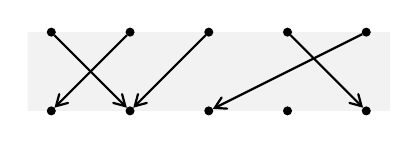
\begin{tikzpicture}
\tikzstyle{blackdot}=[draw=black,circle,fill=black,inner sep=1pt]
\tikzstyle{arrow}=[thick,->,>=angle 60]
\node [blackdot] at (0,0) (u1) {};
\node [blackdot,right of=u1] (u2) {};
\node [blackdot,right of=u2] (u3) {};
\node [blackdot,right of=u3] (u4) {};
\node [blackdot,right of=u4] (u5) {};
\node [blackdot,below of=u1] (d1) {};
\node [blackdot,below of=u2] (d2) {};
\node [blackdot,below of=u3] (d3) {};
\node [blackdot,below of=u4] (d4) {};
\node [blackdot,below of=u5] (d5) {};
\draw [arrow] (u1) edge (d2);
\draw [arrow] (u2) edge (d1);
\draw [arrow] (u3) edge (d2);
\draw [arrow] (u4) edge (d5);
\draw [arrow] (u5) edge (d3);
\begin{pgfonlayer}{background layer}
\fill  [grey] plot (-.3,0) rectangle (4.3,-1);
\end{pgfonlayer}
\end{tikzpicture}
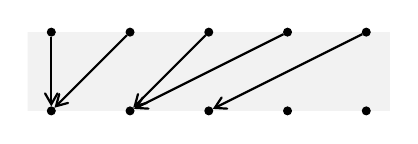
\begin{tikzpicture}
\tikzstyle{blackdot}=[draw=black,circle,fill=black,inner sep=1pt]
\tikzstyle{arrow}=[thick,->,>=angle 60]
\node [blackdot] at (0,0) (u1) {};
\node [blackdot,right of=u1] (u2) {};
\node [blackdot,right of=u2] (u3) {};
\node [blackdot,right of=u3] (u4) {};
\node [blackdot,right of=u4] (u5) {};
\node [blackdot,below of=u1] (d1) {};
\node [blackdot,below of=u2] (d2) {};
\node [blackdot,below of=u3] (d3) {};
\node [blackdot,below of=u4] (d4) {};
\node [blackdot,below of=u5] (d5) {};
\draw [arrow] (u1) edge (d1);
\draw [arrow] (u2) edge (d1);
\draw [arrow] (u3) edge (d2);
\draw [arrow] (u4) edge (d2);
\draw [arrow] (u5) edge (d3);
\begin{pgfonlayer}{background layer}
\fill  [grey] plot (-.3,0) rectangle (4.3,-1);
\end{pgfonlayer}
\end{tikzpicture}

=

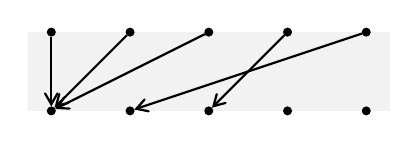
\begin{tikzpicture}
\tikzstyle{blackdot}=[draw=black,circle,fill=black,inner sep=1pt]
\tikzstyle{arrow}=[thick,->,>=angle 60]
\node [blackdot] at (0,0) (u1) {};
\node [blackdot,right of=u1] (u2) {};
\node [blackdot,right of=u2] (u3) {};
\node [blackdot,right of=u3] (u4) {};
\node [blackdot,right of=u4] (u5) {};
\node [blackdot,below of=u1] (d1) {};
\node [blackdot,below of=u2] (d2) {};
\node [blackdot,below of=u3] (d3) {};
\node [blackdot,below of=u4] (d4) {};
\node [blackdot,below of=u5] (d5) {};
\draw [arrow] (u1) edge (d1);
\draw [arrow] (u2) edge (d1);
\draw [arrow] (u3) edge (d1);
\draw [arrow] (u4) edge (d3);
\draw [arrow] (u5) edge (d2);
\begin{pgfonlayer}{background layer}
\fill  [grey] plot (-.3,0) rectangle (4.3,-1);
\end{pgfonlayer}
\end{tikzpicture}
\end{center}
\end{example}
\end{columns}
\end{frame}




\begin{frame}%\frametitle{transformation semigroup}
%A \emph{transformation semigroup}  $(X,S)$ of degree $n$
%is a collection $S$
%of transformations of an $n$-element set $X$
%closed under function composition.
%\gap
\frametitle{Flip-flop, the 1-bit memory semigroup}
\begin{center}
write 0 \hskip2.1cm write 1 \hskip2.1cm read
\scalebox{2}{
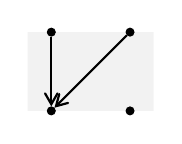
\begin{tikzpicture}
\tikzstyle{blackdot}=[draw=black,circle,fill=black,inner sep=1pt]
\tikzstyle{arrow}=[thick,->,>=angle 60]
\node [blackdot] at (0,0) (u1) {};
\node [blackdot,right of=u1] (u2) {};
\node [blackdot,below of=u1] (d1) {};
\node [blackdot,below of=u2] (d2) {};
\draw [arrow] (u1) edge (d1);
\draw [arrow] (u2) edge (d1);
\begin{pgfonlayer}{background layer}
\fill  [bkg] plot (-.3,0) rectangle (1.3,-1);
\end{pgfonlayer}
\end{tikzpicture}
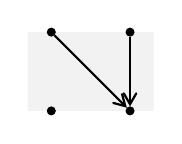
\begin{tikzpicture}
\tikzstyle{blackdot}=[draw=black,circle,fill=black,inner sep=1pt]
\tikzstyle{arrow}=[thick,->,>=angle 60]
\node [blackdot] at (0,0) (u1) {};
\node [blackdot,right of=u1] (u2) {};
\node [blackdot,below of=u1] (d1) {};
\node [blackdot,below of=u2] (d2) {};
\draw [arrow] (u1) edge (d2);
\draw [arrow] (u2) edge (d2);
\begin{pgfonlayer}{background layer}
\fill  [bkg] plot (-.3,0) rectangle (1.3,-1);
\end{pgfonlayer}
\end{tikzpicture}
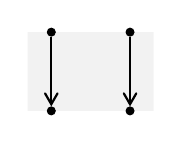
\begin{tikzpicture}
\tikzstyle{blackdot}=[draw=black,circle,fill=black,inner sep=1pt]
\tikzstyle{arrow}=[thick,->,>=angle 60]
\node [blackdot] at (0,0) (u1) {};
\node [blackdot,right of=u1] (u2) {};
\node [blackdot,below of=u1] (d1) {};
\node [blackdot,below of=u2] (d2) {};
\draw [arrow] (u1) edge (d1);
\draw [arrow] (u2) edge (d2);
\begin{pgfonlayer}{background layer}
\fill  [bkg] plot (-.3,0) rectangle (1.3,-1);
\end{pgfonlayer}
\end{tikzpicture}
}

[11] \hskip2.5cm [22] \hskip2.5cm [12]
\end{center}

So these are computational devices... $\approx$ automata
\jump
With transformation semigroups, we get all semigroups. (Cayley's theorem)

%\jump

%AIM: understand their structures
\end{frame}

\begin{frame}\frametitle{Degree 2 transformation semigroups}
\begin{center}
\scalebox{0.8}{
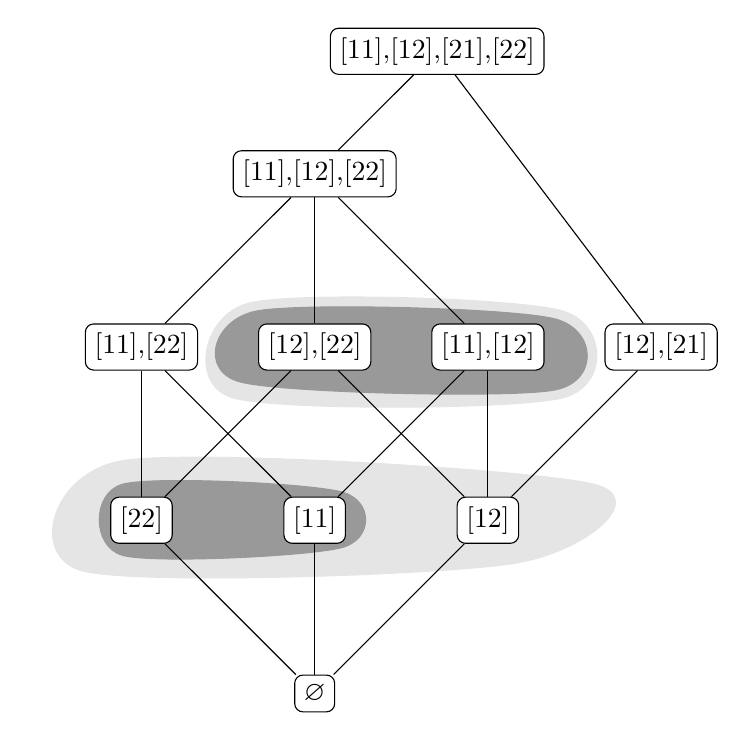
\begin{tikzpicture}
[align=center,node distance=2.2cm]
\tikzstyle{plain}=[fill=white,rounded corners=3pt, draw]


\draw node [plain] (1234) {[11],[12],[21],[22]};
\draw node [plain,below left of=1234] (124) {[11],[12],[22]};
\draw node [plain,below of=124] (24) {[12],[22]};
\draw node [plain,left of=24] (14) {[11],[22]};
\draw node [plain,right of=24] (12) {[11],[12]};
\draw node [plain,right of=12] (23) {[12],[21]};

\draw node [plain,below of=24] (1) {[11]};
\draw node [plain,left of=1] (4) {[22]};
\draw node [plain,right of=1] (2) {[12]};
\draw node [plain,below of=1] (empty) {$\varnothing$};


\draw  (1234) -- (124);
\draw (124) -- (12);
\draw (124) -- (24);
\draw (124) -- (14);
\draw  (1234) -- (23);
\path (23) edge (2);
\draw (1) -- (empty);
\draw (2) -- (empty);
\draw (4) -- (empty);
\draw (14) -- (4);
\draw (14) -- (1);
\draw (12) -- (2);
\draw (12) -- (1);
\draw (24) -- (4);
\draw (24) -- (2);
\begin{pgfonlayer}{background layer}
\filldraw [gray9] plot [smooth cycle] coordinates {(1.6,-4.4)(-2.6,-4.4) (-2.4,-3.2) (1.6,-3.3)};
\filldraw [gray6] plot [smooth cycle] coordinates {(1.5,-4.3)(-2.5,-4.2) (-2.3,-3.3) (1.5,-3.4)};
\filldraw [gray9] plot [smooth cycle] coordinates {(-4,-5.2) (2,-5.5) (1,-6.5)(-4.5,-6.6)};
\filldraw [gray6] plot [smooth cycle] coordinates {(-4,-5.5) (-1.2,-5.6) (-1.2,-6.3)(-4,-6.4)};

\end{pgfonlayer}

\end{tikzpicture}
}
\end{center}
\end{frame}

\begin{frame}\frametitle{Data flood}

Number of subsemigroups of full transformation semigroups.

\gap
\footnotesize
\renewcommand{\arraystretch}{1}
\begin{tabular}{|c|r|r|r|}
\hline
 & \#subsemigroups & \#conjugacy classes & \#isomorphism classes \\
\hline
$\cT_0$ & 1  & 1 & 1\\
\hline
$\cT_1$ & 2  & 2 & 2\\
\hline
$\cT_2$ & 10  & 8& 7\\
\hline
$\cT_3$ & 1 299 & 283 & 267\\
\hline
$\cT_4$ & 3 161 965 550 & 132 069 776& 131 852 491\\
\hline
\end{tabular}
\normalsize
\gap
After discounting the state-relabelling symmetries the  database of degree 4 transformation semigroups is still around 9GB.
\end{frame}

\begin{frame}\frametitle{Size distribution}
  \scalebox{0.8}{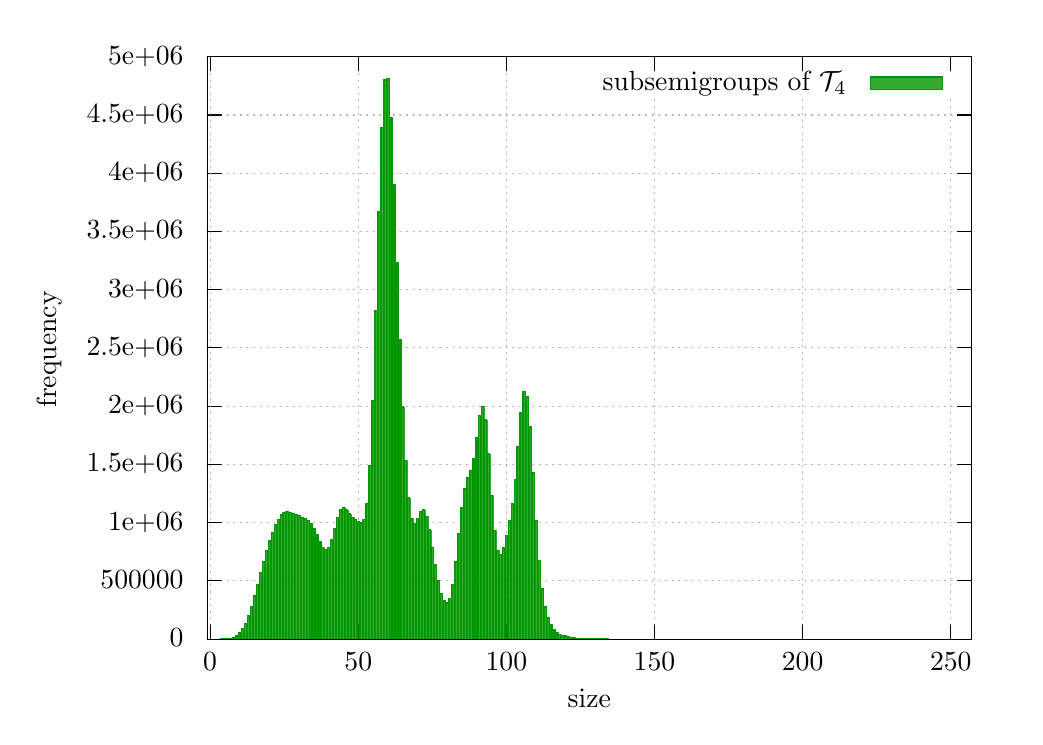
\begin{tikzpicture}[gnuplot]
%% generated with GNUPLOT 4.6p5 (Lua 5.1; terminal rev. 99, script rev. 100)
%% Sat 08 Nov 2014 18:26:18 AEDT
\path (0.000,0.000) rectangle (12.500,8.750);
\gpcolor{color=gp lt color axes}
\gpsetlinetype{gp lt axes}
\gpsetlinewidth{1.00}
\draw[gp path] (2.240,0.985)--(11.947,0.985);
\gpcolor{color=gp lt color border}
\gpsetlinetype{gp lt border}
\draw[gp path] (2.240,0.985)--(2.420,0.985);
\draw[gp path] (11.947,0.985)--(11.767,0.985);
\node[gp node right] at (2.056,0.985) { 0};
\gpcolor{color=gp lt color axes}
\gpsetlinetype{gp lt axes}
\draw[gp path] (2.240,1.725)--(11.947,1.725);
\gpcolor{color=gp lt color border}
\gpsetlinetype{gp lt border}
\draw[gp path] (2.240,1.725)--(2.420,1.725);
\draw[gp path] (11.947,1.725)--(11.767,1.725);
\node[gp node right] at (2.056,1.725) { 500000};
\gpcolor{color=gp lt color axes}
\gpsetlinetype{gp lt axes}
\draw[gp path] (2.240,2.464)--(11.947,2.464);
\gpcolor{color=gp lt color border}
\gpsetlinetype{gp lt border}
\draw[gp path] (2.240,2.464)--(2.420,2.464);
\draw[gp path] (11.947,2.464)--(11.767,2.464);
\node[gp node right] at (2.056,2.464) { 1e+06};
\gpcolor{color=gp lt color axes}
\gpsetlinetype{gp lt axes}
\draw[gp path] (2.240,3.204)--(11.947,3.204);
\gpcolor{color=gp lt color border}
\gpsetlinetype{gp lt border}
\draw[gp path] (2.240,3.204)--(2.420,3.204);
\draw[gp path] (11.947,3.204)--(11.767,3.204);
\node[gp node right] at (2.056,3.204) { 1.5e+06};
\gpcolor{color=gp lt color axes}
\gpsetlinetype{gp lt axes}
\draw[gp path] (2.240,3.943)--(11.947,3.943);
\gpcolor{color=gp lt color border}
\gpsetlinetype{gp lt border}
\draw[gp path] (2.240,3.943)--(2.420,3.943);
\draw[gp path] (11.947,3.943)--(11.767,3.943);
\node[gp node right] at (2.056,3.943) { 2e+06};
\gpcolor{color=gp lt color axes}
\gpsetlinetype{gp lt axes}
\draw[gp path] (2.240,4.683)--(11.947,4.683);
\gpcolor{color=gp lt color border}
\gpsetlinetype{gp lt border}
\draw[gp path] (2.240,4.683)--(2.420,4.683);
\draw[gp path] (11.947,4.683)--(11.767,4.683);
\node[gp node right] at (2.056,4.683) { 2.5e+06};
\gpcolor{color=gp lt color axes}
\gpsetlinetype{gp lt axes}
\draw[gp path] (2.240,5.423)--(11.947,5.423);
\gpcolor{color=gp lt color border}
\gpsetlinetype{gp lt border}
\draw[gp path] (2.240,5.423)--(2.420,5.423);
\draw[gp path] (11.947,5.423)--(11.767,5.423);
\node[gp node right] at (2.056,5.423) { 3e+06};
\gpcolor{color=gp lt color axes}
\gpsetlinetype{gp lt axes}
\draw[gp path] (2.240,6.162)--(11.947,6.162);
\gpcolor{color=gp lt color border}
\gpsetlinetype{gp lt border}
\draw[gp path] (2.240,6.162)--(2.420,6.162);
\draw[gp path] (11.947,6.162)--(11.767,6.162);
\node[gp node right] at (2.056,6.162) { 3.5e+06};
\gpcolor{color=gp lt color axes}
\gpsetlinetype{gp lt axes}
\draw[gp path] (2.240,6.902)--(11.947,6.902);
\gpcolor{color=gp lt color border}
\gpsetlinetype{gp lt border}
\draw[gp path] (2.240,6.902)--(2.420,6.902);
\draw[gp path] (11.947,6.902)--(11.767,6.902);
\node[gp node right] at (2.056,6.902) { 4e+06};
\gpcolor{color=gp lt color axes}
\gpsetlinetype{gp lt axes}
\draw[gp path] (2.240,7.641)--(11.947,7.641);
\gpcolor{color=gp lt color border}
\gpsetlinetype{gp lt border}
\draw[gp path] (2.240,7.641)--(2.420,7.641);
\draw[gp path] (11.947,7.641)--(11.767,7.641);
\node[gp node right] at (2.056,7.641) { 4.5e+06};
\gpcolor{color=gp lt color axes}
\gpsetlinetype{gp lt axes}
\draw[gp path] (2.240,8.381)--(11.947,8.381);
\gpcolor{color=gp lt color border}
\gpsetlinetype{gp lt border}
\draw[gp path] (2.240,8.381)--(2.420,8.381);
\draw[gp path] (11.947,8.381)--(11.767,8.381);
\node[gp node right] at (2.056,8.381) { 5e+06};
\gpcolor{color=gp lt color axes}
\gpsetlinetype{gp lt axes}
\draw[gp path] (2.278,0.985)--(2.278,8.381);
\gpcolor{color=gp lt color border}
\gpsetlinetype{gp lt border}
\draw[gp path] (2.278,0.985)--(2.278,1.165);
\draw[gp path] (2.278,8.381)--(2.278,8.201);
\node[gp node center] at (2.278,0.677) { 0};
\gpcolor{color=gp lt color axes}
\gpsetlinetype{gp lt axes}
\draw[gp path] (4.159,0.985)--(4.159,8.381);
\gpcolor{color=gp lt color border}
\gpsetlinetype{gp lt border}
\draw[gp path] (4.159,0.985)--(4.159,1.165);
\draw[gp path] (4.159,8.381)--(4.159,8.201);
\node[gp node center] at (4.159,0.677) { 50};
\gpcolor{color=gp lt color axes}
\gpsetlinetype{gp lt axes}
\draw[gp path] (6.040,0.985)--(6.040,8.381);
\gpcolor{color=gp lt color border}
\gpsetlinetype{gp lt border}
\draw[gp path] (6.040,0.985)--(6.040,1.165);
\draw[gp path] (6.040,8.381)--(6.040,8.201);
\node[gp node center] at (6.040,0.677) { 100};
\gpcolor{color=gp lt color axes}
\gpsetlinetype{gp lt axes}
\draw[gp path] (7.921,0.985)--(7.921,7.893);
\draw[gp path] (7.921,8.201)--(7.921,8.381);
\gpcolor{color=gp lt color border}
\gpsetlinetype{gp lt border}
\draw[gp path] (7.921,0.985)--(7.921,1.165);
\draw[gp path] (7.921,8.381)--(7.921,8.201);
\node[gp node center] at (7.921,0.677) { 150};
\gpcolor{color=gp lt color axes}
\gpsetlinetype{gp lt axes}
\draw[gp path] (9.802,0.985)--(9.802,7.893);
\draw[gp path] (9.802,8.201)--(9.802,8.381);
\gpcolor{color=gp lt color border}
\gpsetlinetype{gp lt border}
\draw[gp path] (9.802,0.985)--(9.802,1.165);
\draw[gp path] (9.802,8.381)--(9.802,8.201);
\node[gp node center] at (9.802,0.677) { 200};
\gpcolor{color=gp lt color axes}
\gpsetlinetype{gp lt axes}
\draw[gp path] (11.684,0.985)--(11.684,7.893);
\draw[gp path] (11.684,8.201)--(11.684,8.381);
\gpcolor{color=gp lt color border}
\gpsetlinetype{gp lt border}
\draw[gp path] (11.684,0.985)--(11.684,1.165);
\draw[gp path] (11.684,8.381)--(11.684,8.201);
\node[gp node center] at (11.684,0.677) { 250};
\draw[gp path] (2.240,8.381)--(2.240,0.985)--(11.947,0.985)--(11.947,8.381)--cycle;
\node[gp node center,rotate=-270] at (0.246,4.683) {frequency};
\node[gp node center] at (7.093,0.215) {size};
\node[gp node right] at (10.479,8.047) {subsemigroups of ${\cal T}_4$};
\gpfill{rgb color={0.000,0.588,0.000},opacity=0.80} (10.663,7.970)--(11.579,7.970)--(11.579,8.124)--(10.663,8.124)--cycle;
\gpcolor{rgb color={0.000,0.588,0.000}}
\gpsetlinetype{gp lt plot 0}
\draw[gp path] (10.663,7.970)--(11.579,7.970)--(11.579,8.124)--(10.663,8.124)--cycle;
\gpfill{rgb color={0.000,0.588,0.000},opacity=0.80} (2.263,0.985)--(2.294,0.985)--(2.294,0.986)--(2.263,0.986)--cycle;
\draw[gp path] (2.263,0.985)--(2.293,0.985)--cycle;
\gpfill{rgb color={0.000,0.588,0.000},opacity=0.80} (2.300,0.985)--(2.331,0.985)--(2.331,0.986)--(2.300,0.986)--cycle;
\draw[gp path] (2.300,0.985)--(2.330,0.985)--cycle;
\gpfill{rgb color={0.000,0.588,0.000},opacity=0.80} (2.338,0.985)--(2.369,0.985)--(2.369,0.986)--(2.338,0.986)--cycle;
\draw[gp path] (2.338,0.985)--(2.368,0.985)--cycle;
\gpfill{rgb color={0.000,0.588,0.000},opacity=0.80} (2.375,0.985)--(2.407,0.985)--(2.407,0.986)--(2.375,0.986)--cycle;
\draw[gp path] (2.375,0.985)--(2.406,0.985)--cycle;
\gpfill{rgb color={0.000,0.588,0.000},opacity=0.80} (2.413,0.985)--(2.444,0.985)--(2.444,0.987)--(2.413,0.987)--cycle;
\draw[gp path] (2.413,0.985)--(2.413,0.986)--(2.443,0.986)--(2.443,0.985)--cycle;
\gpfill{rgb color={0.000,0.588,0.000},opacity=0.80} (2.451,0.985)--(2.482,0.985)--(2.482,0.988)--(2.451,0.988)--cycle;
\draw[gp path] (2.451,0.985)--(2.451,0.987)--(2.481,0.987)--(2.481,0.985)--cycle;
\gpfill{rgb color={0.000,0.588,0.000},opacity=0.80} (2.488,0.985)--(2.519,0.985)--(2.519,0.990)--(2.488,0.990)--cycle;
\draw[gp path] (2.488,0.985)--(2.488,0.989)--(2.518,0.989)--(2.518,0.985)--cycle;
\gpfill{rgb color={0.000,0.588,0.000},opacity=0.80} (2.526,0.985)--(2.557,0.985)--(2.557,0.996)--(2.526,0.996)--cycle;
\draw[gp path] (2.526,0.985)--(2.526,0.995)--(2.556,0.995)--(2.556,0.985)--cycle;
\gpfill{rgb color={0.000,0.588,0.000},opacity=0.80} (2.564,0.985)--(2.595,0.985)--(2.595,1.008)--(2.564,1.008)--cycle;
\draw[gp path] (2.564,0.985)--(2.564,1.007)--(2.594,1.007)--(2.594,0.985)--cycle;
\gpfill{rgb color={0.000,0.588,0.000},opacity=0.80} (2.601,0.985)--(2.632,0.985)--(2.632,1.029)--(2.601,1.029)--cycle;
\draw[gp path] (2.601,0.985)--(2.601,1.028)--(2.631,1.028)--(2.631,0.985)--cycle;
\gpfill{rgb color={0.000,0.588,0.000},opacity=0.80} (2.639,0.985)--(2.670,0.985)--(2.670,1.063)--(2.639,1.063)--cycle;
\draw[gp path] (2.639,0.985)--(2.639,1.062)--(2.669,1.062)--(2.669,0.985)--cycle;
\gpfill{rgb color={0.000,0.588,0.000},opacity=0.80} (2.676,0.985)--(2.708,0.985)--(2.708,1.114)--(2.676,1.114)--cycle;
\draw[gp path] (2.676,0.985)--(2.676,1.113)--(2.707,1.113)--(2.707,0.985)--cycle;
\gpfill{rgb color={0.000,0.588,0.000},opacity=0.80} (2.714,0.985)--(2.745,0.985)--(2.745,1.187)--(2.714,1.187)--cycle;
\draw[gp path] (2.714,0.985)--(2.714,1.186)--(2.744,1.186)--(2.744,0.985)--cycle;
\gpfill{rgb color={0.000,0.588,0.000},opacity=0.80} (2.752,0.985)--(2.783,0.985)--(2.783,1.283)--(2.752,1.283)--cycle;
\draw[gp path] (2.752,0.985)--(2.752,1.282)--(2.782,1.282)--(2.782,0.985)--cycle;
\gpfill{rgb color={0.000,0.588,0.000},opacity=0.80} (2.789,0.985)--(2.820,0.985)--(2.820,1.401)--(2.789,1.401)--cycle;
\draw[gp path] (2.789,0.985)--(2.789,1.400)--(2.819,1.400)--(2.819,0.985)--cycle;
\gpfill{rgb color={0.000,0.588,0.000},opacity=0.80} (2.827,0.985)--(2.858,0.985)--(2.858,1.535)--(2.827,1.535)--cycle;
\draw[gp path] (2.827,0.985)--(2.827,1.534)--(2.857,1.534)--(2.857,0.985)--cycle;
\gpfill{rgb color={0.000,0.588,0.000},opacity=0.80} (2.865,0.985)--(2.896,0.985)--(2.896,1.681)--(2.865,1.681)--cycle;
\draw[gp path] (2.865,0.985)--(2.865,1.680)--(2.895,1.680)--(2.895,0.985)--cycle;
\gpfill{rgb color={0.000,0.588,0.000},opacity=0.80} (2.902,0.985)--(2.933,0.985)--(2.933,1.829)--(2.902,1.829)--cycle;
\draw[gp path] (2.902,0.985)--(2.902,1.828)--(2.932,1.828)--(2.932,0.985)--cycle;
\gpfill{rgb color={0.000,0.588,0.000},opacity=0.80} (2.940,0.985)--(2.971,0.985)--(2.971,1.977)--(2.940,1.977)--cycle;
\draw[gp path] (2.940,0.985)--(2.940,1.976)--(2.970,1.976)--(2.970,0.985)--cycle;
\gpfill{rgb color={0.000,0.588,0.000},opacity=0.80} (2.977,0.985)--(3.009,0.985)--(3.009,2.114)--(2.977,2.114)--cycle;
\draw[gp path] (2.977,0.985)--(2.977,2.113)--(3.008,2.113)--(3.008,0.985)--cycle;
\gpfill{rgb color={0.000,0.588,0.000},opacity=0.80} (3.015,0.985)--(3.046,0.985)--(3.046,2.239)--(3.015,2.239)--cycle;
\draw[gp path] (3.015,0.985)--(3.015,2.238)--(3.045,2.238)--(3.045,0.985)--cycle;
\gpfill{rgb color={0.000,0.588,0.000},opacity=0.80} (3.053,0.985)--(3.084,0.985)--(3.084,2.345)--(3.053,2.345)--cycle;
\draw[gp path] (3.053,0.985)--(3.053,2.344)--(3.083,2.344)--(3.083,0.985)--cycle;
\gpfill{rgb color={0.000,0.588,0.000},opacity=0.80} (3.090,0.985)--(3.121,0.985)--(3.121,2.437)--(3.090,2.437)--cycle;
\draw[gp path] (3.090,0.985)--(3.090,2.436)--(3.120,2.436)--(3.120,0.985)--cycle;
\gpfill{rgb color={0.000,0.588,0.000},opacity=0.80} (3.128,0.985)--(3.159,0.985)--(3.159,2.507)--(3.128,2.507)--cycle;
\draw[gp path] (3.128,0.985)--(3.128,2.506)--(3.158,2.506)--(3.158,0.985)--cycle;
\gpfill{rgb color={0.000,0.588,0.000},opacity=0.80} (3.166,0.985)--(3.197,0.985)--(3.197,2.562)--(3.166,2.562)--cycle;
\draw[gp path] (3.166,0.985)--(3.166,2.561)--(3.196,2.561)--(3.196,0.985)--cycle;
\gpfill{rgb color={0.000,0.588,0.000},opacity=0.80} (3.203,0.985)--(3.234,0.985)--(3.234,2.591)--(3.203,2.591)--cycle;
\draw[gp path] (3.203,0.985)--(3.203,2.590)--(3.233,2.590)--(3.233,0.985)--cycle;
\gpfill{rgb color={0.000,0.588,0.000},opacity=0.80} (3.241,0.985)--(3.272,0.985)--(3.272,2.602)--(3.241,2.602)--cycle;
\draw[gp path] (3.241,0.985)--(3.241,2.601)--(3.271,2.601)--(3.271,0.985)--cycle;
\gpfill{rgb color={0.000,0.588,0.000},opacity=0.80} (3.278,0.985)--(3.310,0.985)--(3.310,2.594)--(3.278,2.594)--cycle;
\draw[gp path] (3.278,0.985)--(3.278,2.593)--(3.309,2.593)--(3.309,0.985)--cycle;
\gpfill{rgb color={0.000,0.588,0.000},opacity=0.80} (3.316,0.985)--(3.347,0.985)--(3.347,2.581)--(3.316,2.581)--cycle;
\draw[gp path] (3.316,0.985)--(3.316,2.580)--(3.346,2.580)--(3.346,0.985)--cycle;
\gpfill{rgb color={0.000,0.588,0.000},opacity=0.80} (3.354,0.985)--(3.385,0.985)--(3.385,2.563)--(3.354,2.563)--cycle;
\draw[gp path] (3.354,0.985)--(3.354,2.562)--(3.384,2.562)--(3.384,0.985)--cycle;
\gpfill{rgb color={0.000,0.588,0.000},opacity=0.80} (3.391,0.985)--(3.422,0.985)--(3.422,2.550)--(3.391,2.550)--cycle;
\draw[gp path] (3.391,0.985)--(3.391,2.549)--(3.421,2.549)--(3.421,0.985)--cycle;
\gpfill{rgb color={0.000,0.588,0.000},opacity=0.80} (3.429,0.985)--(3.460,0.985)--(3.460,2.533)--(3.429,2.533)--cycle;
\draw[gp path] (3.429,0.985)--(3.429,2.532)--(3.459,2.532)--(3.459,0.985)--cycle;
\gpfill{rgb color={0.000,0.588,0.000},opacity=0.80} (3.467,0.985)--(3.498,0.985)--(3.498,2.519)--(3.467,2.519)--cycle;
\draw[gp path] (3.467,0.985)--(3.467,2.518)--(3.497,2.518)--(3.497,0.985)--cycle;
\gpfill{rgb color={0.000,0.588,0.000},opacity=0.80} (3.504,0.985)--(3.535,0.985)--(3.535,2.492)--(3.504,2.492)--cycle;
\draw[gp path] (3.504,0.985)--(3.504,2.491)--(3.534,2.491)--(3.534,0.985)--cycle;
\gpfill{rgb color={0.000,0.588,0.000},opacity=0.80} (3.542,0.985)--(3.573,0.985)--(3.573,2.454)--(3.542,2.454)--cycle;
\draw[gp path] (3.542,0.985)--(3.542,2.453)--(3.572,2.453)--(3.572,0.985)--cycle;
\gpfill{rgb color={0.000,0.588,0.000},opacity=0.80} (3.579,0.985)--(3.611,0.985)--(3.611,2.389)--(3.579,2.389)--cycle;
\draw[gp path] (3.579,0.985)--(3.579,2.388)--(3.610,2.388)--(3.610,0.985)--cycle;
\gpfill{rgb color={0.000,0.588,0.000},opacity=0.80} (3.617,0.985)--(3.648,0.985)--(3.648,2.309)--(3.617,2.309)--cycle;
\draw[gp path] (3.617,0.985)--(3.617,2.308)--(3.647,2.308)--(3.647,0.985)--cycle;
\gpfill{rgb color={0.000,0.588,0.000},opacity=0.80} (3.655,0.985)--(3.686,0.985)--(3.686,2.220)--(3.655,2.220)--cycle;
\draw[gp path] (3.655,0.985)--(3.655,2.219)--(3.685,2.219)--(3.685,0.985)--cycle;
\gpfill{rgb color={0.000,0.588,0.000},opacity=0.80} (3.692,0.985)--(3.723,0.985)--(3.723,2.152)--(3.692,2.152)--cycle;
\draw[gp path] (3.692,0.985)--(3.692,2.151)--(3.722,2.151)--(3.722,0.985)--cycle;
\gpfill{rgb color={0.000,0.588,0.000},opacity=0.80} (3.730,0.985)--(3.761,0.985)--(3.761,2.120)--(3.730,2.120)--cycle;
\draw[gp path] (3.730,0.985)--(3.730,2.119)--(3.760,2.119)--(3.760,0.985)--cycle;
\gpfill{rgb color={0.000,0.588,0.000},opacity=0.80} (3.768,0.985)--(3.799,0.985)--(3.799,2.151)--(3.768,2.151)--cycle;
\draw[gp path] (3.768,0.985)--(3.768,2.150)--(3.798,2.150)--(3.798,0.985)--cycle;
\gpfill{rgb color={0.000,0.588,0.000},opacity=0.80} (3.805,0.985)--(3.836,0.985)--(3.836,2.245)--(3.805,2.245)--cycle;
\draw[gp path] (3.805,0.985)--(3.805,2.244)--(3.835,2.244)--(3.835,0.985)--cycle;
\gpfill{rgb color={0.000,0.588,0.000},opacity=0.80} (3.843,0.985)--(3.874,0.985)--(3.874,2.389)--(3.843,2.389)--cycle;
\draw[gp path] (3.843,0.985)--(3.843,2.388)--(3.873,2.388)--(3.873,0.985)--cycle;
\gpfill{rgb color={0.000,0.588,0.000},opacity=0.80} (3.880,0.985)--(3.912,0.985)--(3.912,2.532)--(3.880,2.532)--cycle;
\draw[gp path] (3.880,0.985)--(3.880,2.531)--(3.911,2.531)--(3.911,0.985)--cycle;
\gpfill{rgb color={0.000,0.588,0.000},opacity=0.80} (3.918,0.985)--(3.949,0.985)--(3.949,2.631)--(3.918,2.631)--cycle;
\draw[gp path] (3.918,0.985)--(3.918,2.630)--(3.948,2.630)--(3.948,0.985)--cycle;
\gpfill{rgb color={0.000,0.588,0.000},opacity=0.80} (3.956,0.985)--(3.987,0.985)--(3.987,2.656)--(3.956,2.656)--cycle;
\draw[gp path] (3.956,0.985)--(3.956,2.655)--(3.986,2.655)--(3.986,0.985)--cycle;
\gpfill{rgb color={0.000,0.588,0.000},opacity=0.80} (3.993,0.985)--(4.024,0.985)--(4.024,2.626)--(3.993,2.626)--cycle;
\draw[gp path] (3.993,0.985)--(3.993,2.625)--(4.023,2.625)--(4.023,0.985)--cycle;
\gpfill{rgb color={0.000,0.588,0.000},opacity=0.80} (4.031,0.985)--(4.062,0.985)--(4.062,2.575)--(4.031,2.575)--cycle;
\draw[gp path] (4.031,0.985)--(4.031,2.574)--(4.061,2.574)--(4.061,0.985)--cycle;
\gpfill{rgb color={0.000,0.588,0.000},opacity=0.80} (4.069,0.985)--(4.100,0.985)--(4.100,2.535)--(4.069,2.535)--cycle;
\draw[gp path] (4.069,0.985)--(4.069,2.534)--(4.099,2.534)--(4.099,0.985)--cycle;
\gpfill{rgb color={0.000,0.588,0.000},opacity=0.80} (4.106,0.985)--(4.137,0.985)--(4.137,2.504)--(4.106,2.504)--cycle;
\draw[gp path] (4.106,0.985)--(4.106,2.503)--(4.136,2.503)--(4.136,0.985)--cycle;
\gpfill{rgb color={0.000,0.588,0.000},opacity=0.80} (4.144,0.985)--(4.175,0.985)--(4.175,2.480)--(4.144,2.480)--cycle;
\draw[gp path] (4.144,0.985)--(4.144,2.479)--(4.174,2.479)--(4.174,0.985)--cycle;
\gpfill{rgb color={0.000,0.588,0.000},opacity=0.80} (4.181,0.985)--(4.212,0.985)--(4.212,2.462)--(4.181,2.462)--cycle;
\draw[gp path] (4.181,0.985)--(4.181,2.461)--(4.211,2.461)--(4.211,0.985)--cycle;
\gpfill{rgb color={0.000,0.588,0.000},opacity=0.80} (4.219,0.985)--(4.250,0.985)--(4.250,2.506)--(4.219,2.506)--cycle;
\draw[gp path] (4.219,0.985)--(4.219,2.505)--(4.249,2.505)--(4.249,0.985)--cycle;
\gpfill{rgb color={0.000,0.588,0.000},opacity=0.80} (4.257,0.985)--(4.288,0.985)--(4.288,2.705)--(4.257,2.705)--cycle;
\draw[gp path] (4.257,0.985)--(4.257,2.704)--(4.287,2.704)--(4.287,0.985)--cycle;
\gpfill{rgb color={0.000,0.588,0.000},opacity=0.80} (4.294,0.985)--(4.325,0.985)--(4.325,3.184)--(4.294,3.184)--cycle;
\draw[gp path] (4.294,0.985)--(4.294,3.183)--(4.324,3.183)--(4.324,0.985)--cycle;
\gpfill{rgb color={0.000,0.588,0.000},opacity=0.80} (4.332,0.985)--(4.363,0.985)--(4.363,4.016)--(4.332,4.016)--cycle;
\draw[gp path] (4.332,0.985)--(4.332,4.015)--(4.362,4.015)--(4.362,0.985)--cycle;
\gpfill{rgb color={0.000,0.588,0.000},opacity=0.80} (4.370,0.985)--(4.401,0.985)--(4.401,5.161)--(4.370,5.161)--cycle;
\draw[gp path] (4.370,0.985)--(4.370,5.160)--(4.400,5.160)--(4.400,0.985)--cycle;
\gpfill{rgb color={0.000,0.588,0.000},opacity=0.80} (4.407,0.985)--(4.438,0.985)--(4.438,6.415)--(4.407,6.415)--cycle;
\draw[gp path] (4.407,0.985)--(4.407,6.414)--(4.437,6.414)--(4.437,0.985)--cycle;
\gpfill{rgb color={0.000,0.588,0.000},opacity=0.80} (4.445,0.985)--(4.476,0.985)--(4.476,7.482)--(4.445,7.482)--cycle;
\draw[gp path] (4.445,0.985)--(4.445,7.481)--(4.475,7.481)--(4.475,0.985)--cycle;
\gpfill{rgb color={0.000,0.588,0.000},opacity=0.80} (4.482,0.985)--(4.513,0.985)--(4.513,8.087)--(4.482,8.087)--cycle;
\draw[gp path] (4.482,0.985)--(4.482,8.086)--(4.512,8.086)--(4.512,0.985)--cycle;
\gpfill{rgb color={0.000,0.588,0.000},opacity=0.80} (4.520,0.985)--(4.551,0.985)--(4.551,8.111)--(4.520,8.111)--cycle;
\draw[gp path] (4.520,0.985)--(4.520,8.110)--(4.550,8.110)--(4.550,0.985)--cycle;
\gpfill{rgb color={0.000,0.588,0.000},opacity=0.80} (4.558,0.985)--(4.589,0.985)--(4.589,7.606)--(4.558,7.606)--cycle;
\draw[gp path] (4.558,0.985)--(4.558,7.605)--(4.588,7.605)--(4.588,0.985)--cycle;
\gpfill{rgb color={0.000,0.588,0.000},opacity=0.80} (4.595,0.985)--(4.626,0.985)--(4.626,6.757)--(4.595,6.757)--cycle;
\draw[gp path] (4.595,0.985)--(4.595,6.756)--(4.625,6.756)--(4.625,0.985)--cycle;
\gpfill{rgb color={0.000,0.588,0.000},opacity=0.80} (4.633,0.985)--(4.664,0.985)--(4.664,5.763)--(4.633,5.763)--cycle;
\draw[gp path] (4.633,0.985)--(4.633,5.762)--(4.663,5.762)--(4.663,0.985)--cycle;
\gpfill{rgb color={0.000,0.588,0.000},opacity=0.80} (4.671,0.985)--(4.702,0.985)--(4.702,4.792)--(4.671,4.792)--cycle;
\draw[gp path] (4.671,0.985)--(4.671,4.791)--(4.701,4.791)--(4.701,0.985)--cycle;
\gpfill{rgb color={0.000,0.588,0.000},opacity=0.80} (4.708,0.985)--(4.739,0.985)--(4.739,3.938)--(4.708,3.938)--cycle;
\draw[gp path] (4.708,0.985)--(4.708,3.937)--(4.738,3.937)--(4.738,0.985)--cycle;
\gpfill{rgb color={0.000,0.588,0.000},opacity=0.80} (4.746,0.985)--(4.777,0.985)--(4.777,3.259)--(4.746,3.259)--cycle;
\draw[gp path] (4.746,0.985)--(4.746,3.258)--(4.776,3.258)--(4.776,0.985)--cycle;
\gpfill{rgb color={0.000,0.588,0.000},opacity=0.80} (4.783,0.985)--(4.814,0.985)--(4.814,2.780)--(4.783,2.780)--cycle;
\draw[gp path] (4.783,0.985)--(4.783,2.779)--(4.813,2.779)--(4.813,0.985)--cycle;
\gpfill{rgb color={0.000,0.588,0.000},opacity=0.80} (4.821,0.985)--(4.852,0.985)--(4.852,2.522)--(4.821,2.522)--cycle;
\draw[gp path] (4.821,0.985)--(4.821,2.521)--(4.851,2.521)--(4.851,0.985)--cycle;
\gpfill{rgb color={0.000,0.588,0.000},opacity=0.80} (4.859,0.985)--(4.890,0.985)--(4.890,2.459)--(4.859,2.459)--cycle;
\draw[gp path] (4.859,0.985)--(4.859,2.458)--(4.889,2.458)--(4.889,0.985)--cycle;
\gpfill{rgb color={0.000,0.588,0.000},opacity=0.80} (4.896,0.985)--(4.927,0.985)--(4.927,2.523)--(4.896,2.523)--cycle;
\draw[gp path] (4.896,0.985)--(4.896,2.522)--(4.926,2.522)--(4.926,0.985)--cycle;
\gpfill{rgb color={0.000,0.588,0.000},opacity=0.80} (4.934,0.985)--(4.965,0.985)--(4.965,2.608)--(4.934,2.608)--cycle;
\draw[gp path] (4.934,0.985)--(4.934,2.607)--(4.964,2.607)--(4.964,0.985)--cycle;
\gpfill{rgb color={0.000,0.588,0.000},opacity=0.80} (4.972,0.985)--(5.003,0.985)--(5.003,2.630)--(4.972,2.630)--cycle;
\draw[gp path] (4.972,0.985)--(4.972,2.629)--(5.002,2.629)--(5.002,0.985)--cycle;
\gpfill{rgb color={0.000,0.588,0.000},opacity=0.80} (5.009,0.985)--(5.040,0.985)--(5.040,2.546)--(5.009,2.546)--cycle;
\draw[gp path] (5.009,0.985)--(5.009,2.545)--(5.039,2.545)--(5.039,0.985)--cycle;
\gpfill{rgb color={0.000,0.588,0.000},opacity=0.80} (5.047,0.985)--(5.078,0.985)--(5.078,2.373)--(5.047,2.373)--cycle;
\draw[gp path] (5.047,0.985)--(5.047,2.372)--(5.077,2.372)--(5.077,0.985)--cycle;
\gpfill{rgb color={0.000,0.588,0.000},opacity=0.80} (5.084,0.985)--(5.115,0.985)--(5.115,2.152)--(5.084,2.152)--cycle;
\draw[gp path] (5.084,0.985)--(5.084,2.151)--(5.114,2.151)--(5.114,0.985)--cycle;
\gpfill{rgb color={0.000,0.588,0.000},opacity=0.80} (5.122,0.985)--(5.153,0.985)--(5.153,1.927)--(5.122,1.927)--cycle;
\draw[gp path] (5.122,0.985)--(5.122,1.926)--(5.152,1.926)--(5.152,0.985)--cycle;
\gpfill{rgb color={0.000,0.588,0.000},opacity=0.80} (5.160,0.985)--(5.191,0.985)--(5.191,1.725)--(5.160,1.725)--cycle;
\draw[gp path] (5.160,0.985)--(5.160,1.724)--(5.190,1.724)--(5.190,0.985)--cycle;
\gpfill{rgb color={0.000,0.588,0.000},opacity=0.80} (5.197,0.985)--(5.228,0.985)--(5.228,1.570)--(5.197,1.570)--cycle;
\draw[gp path] (5.197,0.985)--(5.197,1.569)--(5.227,1.569)--(5.227,0.985)--cycle;
\gpfill{rgb color={0.000,0.588,0.000},opacity=0.80} (5.235,0.985)--(5.266,0.985)--(5.266,1.473)--(5.235,1.473)--cycle;
\draw[gp path] (5.235,0.985)--(5.235,1.472)--(5.265,1.472)--(5.265,0.985)--cycle;
\gpfill{rgb color={0.000,0.588,0.000},opacity=0.80} (5.272,0.985)--(5.304,0.985)--(5.304,1.444)--(5.272,1.444)--cycle;
\draw[gp path] (5.272,0.985)--(5.272,1.443)--(5.303,1.443)--(5.303,0.985)--cycle;
\gpfill{rgb color={0.000,0.588,0.000},opacity=0.80} (5.310,0.985)--(5.341,0.985)--(5.341,1.504)--(5.310,1.504)--cycle;
\draw[gp path] (5.310,0.985)--(5.310,1.503)--(5.340,1.503)--(5.340,0.985)--cycle;
\gpfill{rgb color={0.000,0.588,0.000},opacity=0.80} (5.348,0.985)--(5.379,0.985)--(5.379,1.680)--(5.348,1.680)--cycle;
\draw[gp path] (5.348,0.985)--(5.348,1.679)--(5.378,1.679)--(5.378,0.985)--cycle;
\gpfill{rgb color={0.000,0.588,0.000},opacity=0.80} (5.385,0.985)--(5.416,0.985)--(5.416,1.969)--(5.385,1.969)--cycle;
\draw[gp path] (5.385,0.985)--(5.385,1.968)--(5.415,1.968)--(5.415,0.985)--cycle;
\gpfill{rgb color={0.000,0.588,0.000},opacity=0.80} (5.423,0.985)--(5.454,0.985)--(5.454,2.320)--(5.423,2.320)--cycle;
\draw[gp path] (5.423,0.985)--(5.423,2.319)--(5.453,2.319)--(5.453,0.985)--cycle;
\gpfill{rgb color={0.000,0.588,0.000},opacity=0.80} (5.461,0.985)--(5.492,0.985)--(5.492,2.652)--(5.461,2.652)--cycle;
\draw[gp path] (5.461,0.985)--(5.461,2.651)--(5.491,2.651)--(5.491,0.985)--cycle;
\gpfill{rgb color={0.000,0.588,0.000},opacity=0.80} (5.498,0.985)--(5.529,0.985)--(5.529,2.896)--(5.498,2.896)--cycle;
\draw[gp path] (5.498,0.985)--(5.498,2.895)--(5.528,2.895)--(5.528,0.985)--cycle;
\gpfill{rgb color={0.000,0.588,0.000},opacity=0.80} (5.536,0.985)--(5.567,0.985)--(5.567,3.033)--(5.536,3.033)--cycle;
\draw[gp path] (5.536,0.985)--(5.536,3.032)--(5.566,3.032)--(5.566,0.985)--cycle;
\gpfill{rgb color={0.000,0.588,0.000},opacity=0.80} (5.573,0.985)--(5.605,0.985)--(5.605,3.126)--(5.573,3.126)--cycle;
\draw[gp path] (5.573,0.985)--(5.573,3.125)--(5.604,3.125)--(5.604,0.985)--cycle;
\gpfill{rgb color={0.000,0.588,0.000},opacity=0.80} (5.611,0.985)--(5.642,0.985)--(5.642,3.277)--(5.611,3.277)--cycle;
\draw[gp path] (5.611,0.985)--(5.611,3.276)--(5.641,3.276)--(5.641,0.985)--cycle;
\gpfill{rgb color={0.000,0.588,0.000},opacity=0.80} (5.649,0.985)--(5.680,0.985)--(5.680,3.542)--(5.649,3.542)--cycle;
\draw[gp path] (5.649,0.985)--(5.649,3.541)--(5.679,3.541)--(5.679,0.985)--cycle;
\gpfill{rgb color={0.000,0.588,0.000},opacity=0.80} (5.686,0.985)--(5.717,0.985)--(5.717,3.825)--(5.686,3.825)--cycle;
\draw[gp path] (5.686,0.985)--(5.686,3.824)--(5.716,3.824)--(5.716,0.985)--cycle;
\gpfill{rgb color={0.000,0.588,0.000},opacity=0.80} (5.724,0.985)--(5.755,0.985)--(5.755,3.944)--(5.724,3.944)--cycle;
\draw[gp path] (5.724,0.985)--(5.724,3.943)--(5.754,3.943)--(5.754,0.985)--cycle;
\gpfill{rgb color={0.000,0.588,0.000},opacity=0.80} (5.762,0.985)--(5.793,0.985)--(5.793,3.770)--(5.762,3.770)--cycle;
\draw[gp path] (5.762,0.985)--(5.762,3.769)--(5.792,3.769)--(5.792,0.985)--cycle;
\gpfill{rgb color={0.000,0.588,0.000},opacity=0.80} (5.799,0.985)--(5.830,0.985)--(5.830,3.340)--(5.799,3.340)--cycle;
\draw[gp path] (5.799,0.985)--(5.799,3.339)--(5.829,3.339)--(5.829,0.985)--cycle;
\gpfill{rgb color={0.000,0.588,0.000},opacity=0.80} (5.837,0.985)--(5.868,0.985)--(5.868,2.813)--(5.837,2.813)--cycle;
\draw[gp path] (5.837,0.985)--(5.837,2.812)--(5.867,2.812)--(5.867,0.985)--cycle;
\gpfill{rgb color={0.000,0.588,0.000},opacity=0.80} (5.874,0.985)--(5.906,0.985)--(5.906,2.369)--(5.874,2.369)--cycle;
\draw[gp path] (5.874,0.985)--(5.874,2.368)--(5.905,2.368)--(5.905,0.985)--cycle;
\gpfill{rgb color={0.000,0.588,0.000},opacity=0.80} (5.912,0.985)--(5.943,0.985)--(5.943,2.115)--(5.912,2.115)--cycle;
\draw[gp path] (5.912,0.985)--(5.912,2.114)--(5.942,2.114)--(5.942,0.985)--cycle;
\gpfill{rgb color={0.000,0.588,0.000},opacity=0.80} (5.950,0.985)--(5.981,0.985)--(5.981,2.059)--(5.950,2.059)--cycle;
\draw[gp path] (5.950,0.985)--(5.950,2.058)--(5.980,2.058)--(5.980,0.985)--cycle;
\gpfill{rgb color={0.000,0.588,0.000},opacity=0.80} (5.987,0.985)--(6.018,0.985)--(6.018,2.147)--(5.987,2.147)--cycle;
\draw[gp path] (5.987,0.985)--(5.987,2.146)--(6.017,2.146)--(6.017,0.985)--cycle;
\gpfill{rgb color={0.000,0.588,0.000},opacity=0.80} (6.025,0.985)--(6.056,0.985)--(6.056,2.306)--(6.025,2.306)--cycle;
\draw[gp path] (6.025,0.985)--(6.025,2.305)--(6.055,2.305)--(6.055,0.985)--cycle;
\gpfill{rgb color={0.000,0.588,0.000},opacity=0.80} (6.063,0.985)--(6.094,0.985)--(6.094,2.487)--(6.063,2.487)--cycle;
\draw[gp path] (6.063,0.985)--(6.063,2.486)--(6.093,2.486)--(6.093,0.985)--cycle;
\gpfill{rgb color={0.000,0.588,0.000},opacity=0.80} (6.100,0.985)--(6.131,0.985)--(6.131,2.702)--(6.100,2.702)--cycle;
\draw[gp path] (6.100,0.985)--(6.100,2.701)--(6.130,2.701)--(6.130,0.985)--cycle;
\gpfill{rgb color={0.000,0.588,0.000},opacity=0.80} (6.138,0.985)--(6.169,0.985)--(6.169,3.007)--(6.138,3.007)--cycle;
\draw[gp path] (6.138,0.985)--(6.138,3.006)--(6.168,3.006)--(6.168,0.985)--cycle;
\gpfill{rgb color={0.000,0.588,0.000},opacity=0.80} (6.175,0.985)--(6.207,0.985)--(6.207,3.430)--(6.175,3.430)--cycle;
\draw[gp path] (6.175,0.985)--(6.175,3.429)--(6.206,3.429)--(6.206,0.985)--cycle;
\gpfill{rgb color={0.000,0.588,0.000},opacity=0.80} (6.213,0.985)--(6.244,0.985)--(6.244,3.865)--(6.213,3.865)--cycle;
\draw[gp path] (6.213,0.985)--(6.213,3.864)--(6.243,3.864)--(6.243,0.985)--cycle;
\gpfill{rgb color={0.000,0.588,0.000},opacity=0.80} (6.251,0.985)--(6.282,0.985)--(6.282,4.130)--(6.251,4.130)--cycle;
\draw[gp path] (6.251,0.985)--(6.251,4.129)--(6.281,4.129)--(6.281,0.985)--cycle;
\gpfill{rgb color={0.000,0.588,0.000},opacity=0.80} (6.288,0.985)--(6.319,0.985)--(6.319,4.067)--(6.288,4.067)--cycle;
\draw[gp path] (6.288,0.985)--(6.288,4.066)--(6.318,4.066)--(6.318,0.985)--cycle;
\gpfill{rgb color={0.000,0.588,0.000},opacity=0.80} (6.326,0.985)--(6.357,0.985)--(6.357,3.681)--(6.326,3.681)--cycle;
\draw[gp path] (6.326,0.985)--(6.326,3.680)--(6.356,3.680)--(6.356,0.985)--cycle;
\gpfill{rgb color={0.000,0.588,0.000},opacity=0.80} (6.364,0.985)--(6.395,0.985)--(6.395,3.096)--(6.364,3.096)--cycle;
\draw[gp path] (6.364,0.985)--(6.364,3.095)--(6.394,3.095)--(6.394,0.985)--cycle;
\gpfill{rgb color={0.000,0.588,0.000},opacity=0.80} (6.401,0.985)--(6.432,0.985)--(6.432,2.490)--(6.401,2.490)--cycle;
\draw[gp path] (6.401,0.985)--(6.401,2.489)--(6.431,2.489)--(6.431,0.985)--cycle;
\gpfill{rgb color={0.000,0.588,0.000},opacity=0.80} (6.439,0.985)--(6.470,0.985)--(6.470,1.986)--(6.439,1.986)--cycle;
\draw[gp path] (6.439,0.985)--(6.439,1.985)--(6.469,1.985)--(6.469,0.985)--cycle;
\gpfill{rgb color={0.000,0.588,0.000},opacity=0.80} (6.476,0.985)--(6.508,0.985)--(6.508,1.626)--(6.476,1.626)--cycle;
\draw[gp path] (6.476,0.985)--(6.476,1.625)--(6.507,1.625)--(6.507,0.985)--cycle;
\gpfill{rgb color={0.000,0.588,0.000},opacity=0.80} (6.514,0.985)--(6.545,0.985)--(6.545,1.397)--(6.514,1.397)--cycle;
\draw[gp path] (6.514,0.985)--(6.514,1.396)--(6.544,1.396)--(6.544,0.985)--cycle;
\gpfill{rgb color={0.000,0.588,0.000},opacity=0.80} (6.552,0.985)--(6.583,0.985)--(6.583,1.254)--(6.552,1.254)--cycle;
\draw[gp path] (6.552,0.985)--(6.552,1.253)--(6.582,1.253)--(6.582,0.985)--cycle;
\gpfill{rgb color={0.000,0.588,0.000},opacity=0.80} (6.589,0.985)--(6.620,0.985)--(6.620,1.167)--(6.589,1.167)--cycle;
\draw[gp path] (6.589,0.985)--(6.589,1.166)--(6.619,1.166)--(6.619,0.985)--cycle;
\gpfill{rgb color={0.000,0.588,0.000},opacity=0.80} (6.627,0.985)--(6.658,0.985)--(6.658,1.109)--(6.627,1.109)--cycle;
\draw[gp path] (6.627,0.985)--(6.627,1.108)--(6.657,1.108)--(6.657,0.985)--cycle;
\gpfill{rgb color={0.000,0.588,0.000},opacity=0.80} (6.665,0.985)--(6.696,0.985)--(6.696,1.072)--(6.665,1.072)--cycle;
\draw[gp path] (6.665,0.985)--(6.665,1.071)--(6.695,1.071)--(6.695,0.985)--cycle;
\gpfill{rgb color={0.000,0.588,0.000},opacity=0.80} (6.702,0.985)--(6.733,0.985)--(6.733,1.048)--(6.702,1.048)--cycle;
\draw[gp path] (6.702,0.985)--(6.702,1.047)--(6.732,1.047)--(6.732,0.985)--cycle;
\gpfill{rgb color={0.000,0.588,0.000},opacity=0.80} (6.740,0.985)--(6.771,0.985)--(6.771,1.035)--(6.740,1.035)--cycle;
\draw[gp path] (6.740,0.985)--(6.740,1.034)--(6.770,1.034)--(6.770,0.985)--cycle;
\gpfill{rgb color={0.000,0.588,0.000},opacity=0.80} (6.777,0.985)--(6.809,0.985)--(6.809,1.025)--(6.777,1.025)--cycle;
\draw[gp path] (6.777,0.985)--(6.777,1.024)--(6.808,1.024)--(6.808,0.985)--cycle;
\gpfill{rgb color={0.000,0.588,0.000},opacity=0.80} (6.815,0.985)--(6.846,0.985)--(6.846,1.017)--(6.815,1.017)--cycle;
\draw[gp path] (6.815,0.985)--(6.815,1.016)--(6.845,1.016)--(6.845,0.985)--cycle;
\gpfill{rgb color={0.000,0.588,0.000},opacity=0.80} (6.853,0.985)--(6.884,0.985)--(6.884,1.009)--(6.853,1.009)--cycle;
\draw[gp path] (6.853,0.985)--(6.853,1.008)--(6.883,1.008)--(6.883,0.985)--cycle;
\gpfill{rgb color={0.000,0.588,0.000},opacity=0.80} (6.890,0.985)--(6.921,0.985)--(6.921,1.002)--(6.890,1.002)--cycle;
\draw[gp path] (6.890,0.985)--(6.890,1.001)--(6.920,1.001)--(6.920,0.985)--cycle;
\gpfill{rgb color={0.000,0.588,0.000},opacity=0.80} (6.928,0.985)--(6.959,0.985)--(6.959,0.998)--(6.928,0.998)--cycle;
\draw[gp path] (6.928,0.985)--(6.928,0.997)--(6.958,0.997)--(6.958,0.985)--cycle;
\gpfill{rgb color={0.000,0.588,0.000},opacity=0.80} (6.966,0.985)--(6.997,0.985)--(6.997,0.994)--(6.966,0.994)--cycle;
\draw[gp path] (6.966,0.985)--(6.966,0.993)--(6.996,0.993)--(6.996,0.985)--cycle;
\gpfill{rgb color={0.000,0.588,0.000},opacity=0.80} (7.003,0.985)--(7.034,0.985)--(7.034,0.992)--(7.003,0.992)--cycle;
\draw[gp path] (7.003,0.985)--(7.003,0.991)--(7.033,0.991)--(7.033,0.985)--cycle;
\gpfill{rgb color={0.000,0.588,0.000},opacity=0.80} (7.041,0.985)--(7.072,0.985)--(7.072,0.990)--(7.041,0.990)--cycle;
\draw[gp path] (7.041,0.985)--(7.041,0.989)--(7.071,0.989)--(7.071,0.985)--cycle;
\gpfill{rgb color={0.000,0.588,0.000},opacity=0.80} (7.078,0.985)--(7.110,0.985)--(7.110,0.989)--(7.078,0.989)--cycle;
\draw[gp path] (7.078,0.985)--(7.078,0.988)--(7.109,0.988)--(7.109,0.985)--cycle;
\gpfill{rgb color={0.000,0.588,0.000},opacity=0.80} (7.116,0.985)--(7.147,0.985)--(7.147,0.989)--(7.116,0.989)--cycle;
\draw[gp path] (7.116,0.985)--(7.116,0.988)--(7.146,0.988)--(7.146,0.985)--cycle;
\gpfill{rgb color={0.000,0.588,0.000},opacity=0.80} (7.154,0.985)--(7.185,0.985)--(7.185,0.989)--(7.154,0.989)--cycle;
\draw[gp path] (7.154,0.985)--(7.154,0.988)--(7.184,0.988)--(7.184,0.985)--cycle;
\gpfill{rgb color={0.000,0.588,0.000},opacity=0.80} (7.191,0.985)--(7.222,0.985)--(7.222,0.988)--(7.191,0.988)--cycle;
\draw[gp path] (7.191,0.985)--(7.191,0.987)--(7.221,0.987)--(7.221,0.985)--cycle;
\gpfill{rgb color={0.000,0.588,0.000},opacity=0.80} (7.229,0.985)--(7.260,0.985)--(7.260,0.987)--(7.229,0.987)--cycle;
\draw[gp path] (7.229,0.985)--(7.229,0.986)--(7.259,0.986)--(7.259,0.985)--cycle;
\gpfill{rgb color={0.000,0.588,0.000},opacity=0.80} (7.267,0.985)--(7.298,0.985)--(7.298,0.987)--(7.267,0.987)--cycle;
\draw[gp path] (7.267,0.985)--(7.267,0.986)--(7.297,0.986)--(7.297,0.985)--cycle;
\gpfill{rgb color={0.000,0.588,0.000},opacity=0.80} (7.304,0.985)--(7.335,0.985)--(7.335,0.987)--(7.304,0.987)--cycle;
\draw[gp path] (7.304,0.985)--(7.304,0.986)--(7.334,0.986)--(7.334,0.985)--cycle;
\gpfill{rgb color={0.000,0.588,0.000},opacity=0.80} (7.342,0.985)--(7.373,0.985)--(7.373,0.986)--(7.342,0.986)--cycle;
\draw[gp path] (7.342,0.985)--(7.372,0.985)--cycle;
\gpfill{rgb color={0.000,0.588,0.000},opacity=0.80} (7.379,0.985)--(7.411,0.985)--(7.411,0.986)--(7.379,0.986)--cycle;
\draw[gp path] (7.379,0.985)--(7.410,0.985)--cycle;
\gpfill{rgb color={0.000,0.588,0.000},opacity=0.80} (7.417,0.985)--(7.448,0.985)--(7.448,0.986)--(7.417,0.986)--cycle;
\draw[gp path] (7.417,0.985)--(7.447,0.985)--cycle;
\gpfill{rgb color={0.000,0.588,0.000},opacity=0.80} (7.455,0.985)--(7.486,0.985)--(7.486,0.986)--(7.455,0.986)--cycle;
\draw[gp path] (7.455,0.985)--(7.485,0.985)--cycle;
\gpfill{rgb color={0.000,0.588,0.000},opacity=0.80} (7.492,0.985)--(7.523,0.985)--(7.523,0.986)--(7.492,0.986)--cycle;
\draw[gp path] (7.492,0.985)--(7.522,0.985)--cycle;
\gpfill{rgb color={0.000,0.588,0.000},opacity=0.80} (7.530,0.985)--(7.561,0.985)--(7.561,0.986)--(7.530,0.986)--cycle;
\draw[gp path] (7.530,0.985)--(7.560,0.985)--cycle;
\gpfill{rgb color={0.000,0.588,0.000},opacity=0.80} (7.568,0.985)--(7.599,0.985)--(7.599,0.986)--(7.568,0.986)--cycle;
\draw[gp path] (7.568,0.985)--(7.598,0.985)--cycle;
\gpfill{rgb color={0.000,0.588,0.000},opacity=0.80} (7.605,0.985)--(7.636,0.985)--(7.636,0.986)--(7.605,0.986)--cycle;
\draw[gp path] (7.605,0.985)--(7.635,0.985)--cycle;
\gpfill{rgb color={0.000,0.588,0.000},opacity=0.80} (7.643,0.985)--(7.674,0.985)--(7.674,0.986)--(7.643,0.986)--cycle;
\draw[gp path] (7.643,0.985)--(7.673,0.985)--cycle;
\gpfill{rgb color={0.000,0.588,0.000},opacity=0.80} (7.680,0.985)--(7.712,0.985)--(7.712,0.986)--(7.680,0.986)--cycle;
\draw[gp path] (7.680,0.985)--(7.711,0.985)--cycle;
\gpfill{rgb color={0.000,0.588,0.000},opacity=0.80} (7.718,0.985)--(7.749,0.985)--(7.749,0.986)--(7.718,0.986)--cycle;
\draw[gp path] (7.718,0.985)--(7.748,0.985)--cycle;
\gpfill{rgb color={0.000,0.588,0.000},opacity=0.80} (7.756,0.985)--(7.787,0.985)--(7.787,0.986)--(7.756,0.986)--cycle;
\draw[gp path] (7.756,0.985)--(7.786,0.985)--cycle;
\gpfill{rgb color={0.000,0.588,0.000},opacity=0.80} (7.793,0.985)--(7.824,0.985)--(7.824,0.986)--(7.793,0.986)--cycle;
\draw[gp path] (7.793,0.985)--(7.823,0.985)--cycle;
\gpfill{rgb color={0.000,0.588,0.000},opacity=0.80} (7.831,0.985)--(7.862,0.985)--(7.862,0.986)--(7.831,0.986)--cycle;
\draw[gp path] (7.831,0.985)--(7.861,0.985)--cycle;
\gpfill{rgb color={0.000,0.588,0.000},opacity=0.80} (7.869,0.985)--(7.900,0.985)--(7.900,0.986)--(7.869,0.986)--cycle;
\draw[gp path] (7.869,0.985)--(7.899,0.985)--cycle;
\gpfill{rgb color={0.000,0.588,0.000},opacity=0.80} (7.906,0.985)--(7.937,0.985)--(7.937,0.986)--(7.906,0.986)--cycle;
\draw[gp path] (7.906,0.985)--(7.936,0.985)--cycle;
\gpfill{rgb color={0.000,0.588,0.000},opacity=0.80} (7.944,0.985)--(7.975,0.985)--(7.975,0.986)--(7.944,0.986)--cycle;
\draw[gp path] (7.944,0.985)--(7.974,0.985)--cycle;
\gpfill{rgb color={0.000,0.588,0.000},opacity=0.80} (7.981,0.985)--(8.013,0.985)--(8.013,0.986)--(7.981,0.986)--cycle;
\draw[gp path] (7.981,0.985)--(8.012,0.985)--cycle;
\gpfill{rgb color={0.000,0.588,0.000},opacity=0.80} (8.019,0.985)--(8.050,0.985)--(8.050,0.986)--(8.019,0.986)--cycle;
\draw[gp path] (8.019,0.985)--(8.049,0.985)--cycle;
\gpfill{rgb color={0.000,0.588,0.000},opacity=0.80} (8.057,0.985)--(8.088,0.985)--(8.088,0.986)--(8.057,0.986)--cycle;
\draw[gp path] (8.057,0.985)--(8.087,0.985)--cycle;
\gpfill{rgb color={0.000,0.588,0.000},opacity=0.80} (8.094,0.985)--(8.125,0.985)--(8.125,0.986)--(8.094,0.986)--cycle;
\draw[gp path] (8.094,0.985)--(8.124,0.985)--cycle;
\gpfill{rgb color={0.000,0.588,0.000},opacity=0.80} (8.132,0.985)--(8.163,0.985)--(8.163,0.986)--(8.132,0.986)--cycle;
\draw[gp path] (8.132,0.985)--(8.162,0.985)--cycle;
\gpfill{rgb color={0.000,0.588,0.000},opacity=0.80} (8.282,0.985)--(8.314,0.985)--(8.314,0.986)--(8.282,0.986)--cycle;
\draw[gp path] (8.282,0.985)--(8.313,0.985)--cycle;
\gpfill{rgb color={0.000,0.588,0.000},opacity=0.80} (8.320,0.985)--(8.351,0.985)--(8.351,0.986)--(8.320,0.986)--cycle;
\draw[gp path] (8.320,0.985)--(8.350,0.985)--cycle;
\gpfill{rgb color={0.000,0.588,0.000},opacity=0.80} (8.358,0.985)--(8.389,0.985)--(8.389,0.986)--(8.358,0.986)--cycle;
\draw[gp path] (8.358,0.985)--(8.388,0.985)--cycle;
\gpfill{rgb color={0.000,0.588,0.000},opacity=0.80} (8.395,0.985)--(8.426,0.985)--(8.426,0.986)--(8.395,0.986)--cycle;
\draw[gp path] (8.395,0.985)--(8.425,0.985)--cycle;
\gpfill{rgb color={0.000,0.588,0.000},opacity=0.80} (8.433,0.985)--(8.464,0.985)--(8.464,0.986)--(8.433,0.986)--cycle;
\draw[gp path] (8.433,0.985)--(8.463,0.985)--cycle;
\gpfill{rgb color={0.000,0.588,0.000},opacity=0.80} (8.471,0.985)--(8.502,0.985)--(8.502,0.986)--(8.471,0.986)--cycle;
\draw[gp path] (8.471,0.985)--(8.501,0.985)--cycle;
\gpfill{rgb color={0.000,0.588,0.000},opacity=0.80} (8.508,0.985)--(8.539,0.985)--(8.539,0.986)--(8.508,0.986)--cycle;
\draw[gp path] (8.508,0.985)--(8.538,0.985)--cycle;
\gpfill{rgb color={0.000,0.588,0.000},opacity=0.80} (8.546,0.985)--(8.577,0.985)--(8.577,0.986)--(8.546,0.986)--cycle;
\draw[gp path] (8.546,0.985)--(8.576,0.985)--cycle;
\gpfill{rgb color={0.000,0.588,0.000},opacity=0.80} (8.583,0.985)--(8.615,0.985)--(8.615,0.986)--(8.583,0.986)--cycle;
\draw[gp path] (8.583,0.985)--(8.614,0.985)--cycle;
\gpfill{rgb color={0.000,0.588,0.000},opacity=0.80} (8.621,0.985)--(8.652,0.985)--(8.652,0.986)--(8.621,0.986)--cycle;
\draw[gp path] (8.621,0.985)--(8.651,0.985)--cycle;
\gpfill{rgb color={0.000,0.588,0.000},opacity=0.80} (8.659,0.985)--(8.690,0.985)--(8.690,0.986)--(8.659,0.986)--cycle;
\draw[gp path] (8.659,0.985)--(8.689,0.985)--cycle;
\gpfill{rgb color={0.000,0.588,0.000},opacity=0.80} (8.734,0.985)--(8.765,0.985)--(8.765,0.986)--(8.734,0.986)--cycle;
\draw[gp path] (8.734,0.985)--(8.764,0.985)--cycle;
\gpfill{rgb color={0.000,0.588,0.000},opacity=0.80} (8.772,0.985)--(8.803,0.985)--(8.803,0.986)--(8.772,0.986)--cycle;
\draw[gp path] (8.772,0.985)--(8.802,0.985)--cycle;
\gpfill{rgb color={0.000,0.588,0.000},opacity=0.80} (8.809,0.985)--(8.840,0.985)--(8.840,0.986)--(8.809,0.986)--cycle;
\draw[gp path] (8.809,0.985)--(8.839,0.985)--cycle;
\gpfill{rgb color={0.000,0.588,0.000},opacity=0.80} (8.884,0.985)--(8.916,0.985)--(8.916,0.986)--(8.884,0.986)--cycle;
\draw[gp path] (8.884,0.985)--(8.915,0.985)--cycle;
\gpfill{rgb color={0.000,0.588,0.000},opacity=0.80} (8.960,0.985)--(8.991,0.985)--(8.991,0.986)--(8.960,0.986)--cycle;
\draw[gp path] (8.960,0.985)--(8.990,0.985)--cycle;
\gpfill{rgb color={0.000,0.588,0.000},opacity=0.80} (8.997,0.985)--(9.028,0.985)--(9.028,0.986)--(8.997,0.986)--cycle;
\draw[gp path] (8.997,0.985)--(9.027,0.985)--cycle;
\gpfill{rgb color={0.000,0.588,0.000},opacity=0.80} (9.035,0.985)--(9.066,0.985)--(9.066,0.986)--(9.035,0.986)--cycle;
\draw[gp path] (9.035,0.985)--(9.065,0.985)--cycle;
\gpfill{rgb color={0.000,0.588,0.000},opacity=0.80} (9.073,0.985)--(9.104,0.985)--(9.104,0.986)--(9.073,0.986)--cycle;
\draw[gp path] (9.073,0.985)--(9.103,0.985)--cycle;
\gpfill{rgb color={0.000,0.588,0.000},opacity=0.80} (9.185,0.985)--(9.216,0.985)--(9.216,0.986)--(9.185,0.986)--cycle;
\draw[gp path] (9.185,0.985)--(9.215,0.985)--cycle;
\gpfill{rgb color={0.000,0.588,0.000},opacity=0.80} (9.223,0.985)--(9.254,0.985)--(9.254,0.986)--(9.223,0.986)--cycle;
\draw[gp path] (9.223,0.985)--(9.253,0.985)--cycle;
\gpfill{rgb color={0.000,0.588,0.000},opacity=0.80} (9.261,0.985)--(9.292,0.985)--(9.292,0.986)--(9.261,0.986)--cycle;
\draw[gp path] (9.261,0.985)--(9.291,0.985)--cycle;
\gpfill{rgb color={0.000,0.588,0.000},opacity=0.80} (9.336,0.985)--(9.367,0.985)--(9.367,0.986)--(9.336,0.986)--cycle;
\draw[gp path] (9.336,0.985)--(9.366,0.985)--cycle;
\gpfill{rgb color={0.000,0.588,0.000},opacity=0.80} (9.486,0.985)--(9.517,0.985)--(9.517,0.986)--(9.486,0.986)--cycle;
\draw[gp path] (9.486,0.985)--(9.516,0.985)--cycle;
\gpfill{rgb color={0.000,0.588,0.000},opacity=0.80} (9.637,0.985)--(9.668,0.985)--(9.668,0.986)--(9.637,0.986)--cycle;
\draw[gp path] (9.637,0.985)--(9.667,0.985)--cycle;
\gpfill{rgb color={0.000,0.588,0.000},opacity=0.80} (9.675,0.985)--(9.706,0.985)--(9.706,0.986)--(9.675,0.986)--cycle;
\draw[gp path] (9.675,0.985)--(9.705,0.985)--cycle;
\gpfill{rgb color={0.000,0.588,0.000},opacity=0.80} (9.712,0.985)--(9.743,0.985)--(9.743,0.986)--(9.712,0.986)--cycle;
\draw[gp path] (9.712,0.985)--(9.742,0.985)--cycle;
\gpfill{rgb color={0.000,0.588,0.000},opacity=0.80} (9.750,0.985)--(9.781,0.985)--(9.781,0.986)--(9.750,0.986)--cycle;
\draw[gp path] (9.750,0.985)--(9.780,0.985)--cycle;
\gpfill{rgb color={0.000,0.588,0.000},opacity=0.80} (9.863,0.985)--(9.894,0.985)--(9.894,0.986)--(9.863,0.986)--cycle;
\draw[gp path] (9.863,0.985)--(9.893,0.985)--cycle;
\gpfill{rgb color={0.000,0.588,0.000},opacity=0.80} (10.088,0.985)--(10.119,0.985)--(10.119,0.986)--(10.088,0.986)--cycle;
\draw[gp path] (10.088,0.985)--(10.118,0.985)--cycle;
\gpfill{rgb color={0.000,0.588,0.000},opacity=0.80} (10.126,0.985)--(10.157,0.985)--(10.157,0.986)--(10.126,0.986)--cycle;
\draw[gp path] (10.126,0.985)--(10.156,0.985)--cycle;
\gpfill{rgb color={0.000,0.588,0.000},opacity=0.80} (10.164,0.985)--(10.195,0.985)--(10.195,0.986)--(10.164,0.986)--cycle;
\draw[gp path] (10.164,0.985)--(10.194,0.985)--cycle;
\gpfill{rgb color={0.000,0.588,0.000},opacity=0.80} (10.239,0.985)--(10.270,0.985)--(10.270,0.986)--(10.239,0.986)--cycle;
\draw[gp path] (10.239,0.985)--(10.269,0.985)--cycle;
\gpfill{rgb color={0.000,0.588,0.000},opacity=0.80} (10.991,0.985)--(11.022,0.985)--(11.022,0.986)--(10.991,0.986)--cycle;
\draw[gp path] (10.991,0.985)--(11.021,0.985)--cycle;
\gpfill{rgb color={0.000,0.588,0.000},opacity=0.80} (11.029,0.985)--(11.060,0.985)--(11.060,0.986)--(11.029,0.986)--cycle;
\draw[gp path] (11.029,0.985)--(11.059,0.985)--cycle;
\gpfill{rgb color={0.000,0.588,0.000},opacity=0.80} (11.067,0.985)--(11.098,0.985)--(11.098,0.986)--(11.067,0.986)--cycle;
\draw[gp path] (11.067,0.985)--(11.097,0.985)--cycle;
\gpfill{rgb color={0.000,0.588,0.000},opacity=0.80} (11.104,0.985)--(11.135,0.985)--(11.135,0.986)--(11.104,0.986)--cycle;
\draw[gp path] (11.104,0.985)--(11.134,0.985)--cycle;
\gpfill{rgb color={0.000,0.588,0.000},opacity=0.80} (11.142,0.985)--(11.173,0.985)--(11.173,0.986)--(11.142,0.986)--cycle;
\draw[gp path] (11.142,0.985)--(11.172,0.985)--cycle;
\gpfill{rgb color={0.000,0.588,0.000},opacity=0.80} (11.217,0.985)--(11.248,0.985)--(11.248,0.986)--(11.217,0.986)--cycle;
\draw[gp path] (11.217,0.985)--(11.247,0.985)--cycle;
\gpfill{rgb color={0.000,0.588,0.000},opacity=0.80} (11.292,0.985)--(11.323,0.985)--(11.323,0.986)--(11.292,0.986)--cycle;
\draw[gp path] (11.292,0.985)--(11.322,0.985)--cycle;
\gpfill{rgb color={0.000,0.588,0.000},opacity=0.80} (11.443,0.985)--(11.474,0.985)--(11.474,0.986)--(11.443,0.986)--cycle;
\draw[gp path] (11.443,0.985)--(11.473,0.985)--cycle;
\gpfill{rgb color={0.000,0.588,0.000},opacity=0.80} (11.894,0.985)--(11.925,0.985)--(11.925,0.986)--(11.894,0.986)--cycle;
\draw[gp path] (11.894,0.985)--(11.924,0.985)--cycle;
\gpcolor{color=gp lt color border}
\gpsetlinetype{gp lt border}
\draw[gp path] (2.240,8.381)--(2.240,0.985)--(11.947,0.985)--(11.947,8.381)--cycle;
%% coordinates of the plot area
\gpdefrectangularnode{gp plot 1}{\pgfpoint{2.240cm}{0.985cm}}{\pgfpoint{11.947cm}{8.381cm}}
\end{tikzpicture}
%% gnuplot variables
}
\end{frame}

\begin{frame}
\begin{figure}
\scalebox{0.75}{
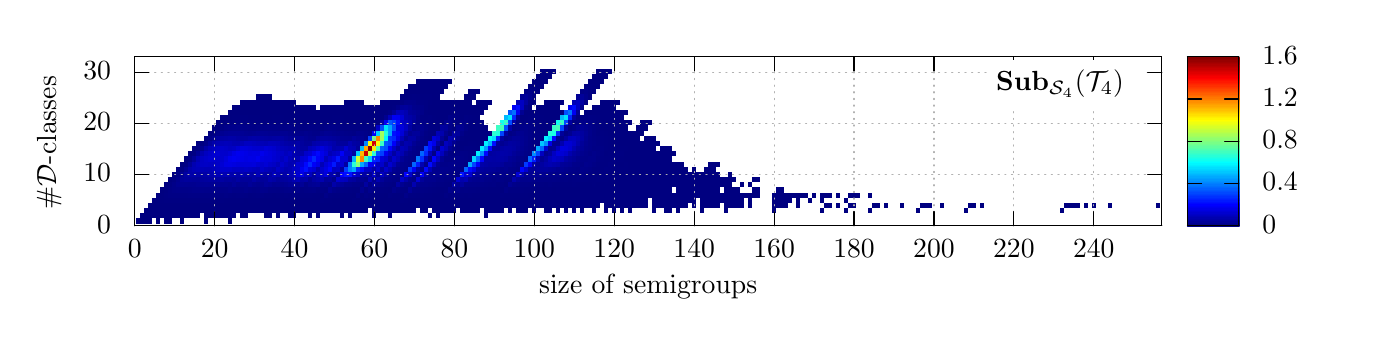
\begin{tikzpicture}[gnuplot]
%% generated with GNUPLOT 4.6p5 (Lua 5.1; terminal rev. 99, script rev. 100)
%% Wed 11 Feb 2015 15:40:24 AEDT
\begin{scope}
\clip (1.320,3.131) rectangle (14.363,0.985);
\def\gprawrgbimagedata{%
  ffffffffffffffffffffffffffffffffffffffffffffffffffffffffffffffffffffffffffffffffffffffffffffffff%
  ffffffffffffffffffffffffffffffffffffffffffffffffffffffffffffffffffffffffffffffffffffffffffffffff%
  ffffffffffffffffffffffffffffffffffffffffffffffffffffffffffffffffffffffffffffffffffffffffffffffff%
  ffffffffffffffffffffffffffffffffffffffffffffffffffffffffffffffffffffffffffffffffffffffffffffffff%
  ffffffffffffffffffffffffffffffffffffffffffffffffffffffffffffffffffffffffffffffffffffffffffffffff%
  ffffffffffffffffffffffffffffffffffffffffffffffffffffffffffffffffffffffffffffffffffffffffffffffff%
  ffffffffffffffffffffffffffffff000080000080000080000080ffffffffffffffffffffffffffffffffffffffffff%
  ffffffffffffffffff000080000080000080000080ffffffffffffffffffffffffffffffffffffffffffffffffffffff%
  ffffffffffffffffffffffffffffffffffffffffffffffffffffffffffffffffffffffffffffffffffffffffffffffff%
  ffffffffffffffffffffffffffffffffffffffffffffffffffffffffffffffffffffffffffffffffffffffffffffffff%
  ffffffffffffffffffffffffffffffffffffffffffffffffffffffffffffffffffffffffffffffffffffffffffffffff%
  ffffffffffffffffffffffffffffffffffffffffffffffffffffffffffffffffffffffffffffffffffffffffffffffff%
  ffffffffffffffffffffffffffffffffffffffffffffffffffffffffffffffffffffffffffffffffffffffffffffffff%
  ffffffffffffffffffffffffffffffffffffffffffffffffffffffffffffffffffffffffffffffffffffffffffffffff%
  ffffffffffffffffffffffffffffffffffffffffffffffffffffffffffffffffffffffffffffffffffffffffffffffff%
  ffffffffffffffffffffffffffffffffffffffffffffffffffffffffffffffffffffffffffffffffffffffffffffffff%
  ffffffffffffffffffffffffffffffffffffffffffffffffffffffffffffffffffffffffffffffffffffffffffffffff%
  ffffffffffffffffffffffffffffffffffffffffffffffffffffffffffffffffffffffffffffffffffffffffffffffff%
  ffffffffffffffffffffffffffffffffffffffffffffffffffffffffffffffffffffffffffffffffffffffffffffffff%
  ffffffffffffffffffffffffffffffffffffffffffffffffffffffffffffffffffffffffffffffffffffffffffffffff%
  ffffffffffffffffffffffffffffffffffffffffffffffffffffffffffffffffffffffffffffffffffffffffffffffff%
  ffffffffffffffffffffffffffffffffffffffffffffffffffffffffffffffffffffffffffffffffffffffffffffffff%
  ffffffffffffffffffffffff000080000080000080000080ffffffffffffffffffffffffffffffffffffffffffffffff%
  ffffffffffff000080000080000080000080ffffffffffffffffffffffffffffffffffffffffffffffffffffffffffff%
  ffffffffffffffffffffffffffffffffffffffffffffffffffffffffffffffffffffffffffffffffffffffffffffffff%
  ffffffffffffffffffffffffffffffffffffffffffffffffffffffffffffffffffffffffffffffffffffffffffffffff%
  ffffffffffffffffffffffffffffffffffffffffffffffffffffffffffffffffffffffffffffffffffffffffffffffff%
  ffffffffffffffffffffffffffffffffffffffffffffffffffffffffffffffffffffffffffffffffffffffffffffffff%
  ffffffffffffffffffffffffffffffffffffffffffffffffffffffffffffffffffffffffffffffffffffffffffffffff%
  ffffffffffffffffffffffffffffffffffffffffffffffffffffffffffffffffffffffffffffffffffffffffffffffff%
  ffffffffffffffffffffffffffffffffffffffffffffffffffffffffffffffffffffffffffffffffffffffffffffffff%
  ffffffffffffffffffffffffffffffffffffffffffffffffffffffffffffffffffffffffffffffffffffffffffffffff%
  ffffffffffffffffffffffffffffffffffffffffffffffffffffffffffffffffffffffffffffffffffffffffffffffff%
  ffffffffffffffffffffffffffffffffffffffffffffffffffffffffffffffffffffffffffffffffffffffffffffffff%
  ffffffffffffffffffffffffffffffffffffffffffffffffffffffffffffffffffffffffffffffffffffffffffffffff%
  ffffffffffffffffffffffffffffffffffffffffffffffffffffffffffffffffffffffffffffffffffffffffffffffff%
  ffffffffffffffffffffffffffffffffffff000080000080000080000080000080000080000080000080000080ffffff%
  ffffffffffffffffffffffffffffffffffffffffffffffffffffffffffffffffffffffffffffffffffffffffffffffff%
  ffffffffffffffffff000080000080000080000080ffffffffffffffffffffffffffffffffffffffffffffffffffffff%
  ffffff000080000080000080000080ffffffffffffffffffffffffffffffffffffffffffffffffffffffffffffffffff%
  ffffffffffffffffffffffffffffffffffffffffffffffffffffffffffffffffffffffffffffffffffffffffffffffff%
  ffffffffffffffffffffffffffffffffffffffffffffffffffffffffffffffffffffffffffffffffffffffffffffffff%
  ffffffffffffffffffffffffffffffffffffffffffffffffffffffffffffffffffffffffffffffffffffffffffffffff%
  ffffffffffffffffffffffffffffffffffffffffffffffffffffffffffffffffffffffffffffffffffffffffffffffff%
  ffffffffffffffffffffffffffffffffffffffffffffffffffffffffffffffffffffffffffffffffffffffffffffffff%
  ffffffffffffffffffffffffffffffffffffffffffffffffffffffffffffffffffffffffffffffffffffffffffffffff%
  ffffffffffffffffffffffffffffffffffffffffffffffffffffffffffffffffffffffffffffffffffffffffffffffff%
  ffffffffffffffffffffffffffffffffffffffffffffffffffffffffffffffffffffffffffffffffffffffffffffffff%
  ffffffffffffffffffffffffffffffffffffffffffffffffffffffffffffffffffffffffffffffffffffffffffffffff%
  ffffffffffffffffffffffffffffffffffffffffffffffffffffffffffffffffffffffffffffffffffffffffffffffff%
  ffffffffffffffffffffffffffffffffffffffffffffffffffffffffffffffffffffffffffffffffffffffffffffffff%
  ffffffffffffffffffffffffffffffffffffffffffffffffffffffffffffffffffffffffffffffffffffffffffffffff%
  ffffffffffffffffffffffff000080000080000080000080000080000080000080000080000080000080ffffffffffff%
  ffffffffffffffffffffffffffffffffffffffffffffffffffffffffffffffffffffffffffffffffffffffffffffffff%
  ffffffffffff000081000082000081000080ffffffffffffffffffffffffffffffffffffffffffffffffffffffffffff%
  000081000082000081000080ffffffffffffffffffffffffffffffffffffffffffffffffffffffffffffffffffffffff%
  ffffffffffffffffffffffffffffffffffffffffffffffffffffffffffffffffffffffffffffffffffffffffffffffff%
  ffffffffffffffffffffffffffffffffffffffffffffffffffffffffffffffffffffffffffffffffffffffffffffffff%
  ffffffffffffffffffffffffffffffffffffffffffffffffffffffffffffffffffffffffffffffffffffffffffffffff%
  ffffffffffffffffffffffffffffffffffffffffffffffffffffffffffffffffffffffffffffffffffffffffffffffff%
  ffffffffffffffffffffffffffffffffffffffffffffffffffffffffffffffffffffffffffffffffffffffffffffffff%
  ffffffffffffffffffffffffffffffffffffffffffffffffffffffffffffffffffffffffffffffffffffffffffffffff%
  ffffffffffffffffffffffffffffffffffffffffffffffffffffffffffffffffffffffffffffffffffffffffffffffff%
  ffffffffffffffffffffffffffffffffffffffffffffffffffffffffffffffffffffffffffffffffffffffffffffffff%
  ffffffffffffffffffffffffffffffffffffffffffffffffffffffffffffffffffffffffffffffffffffffffffffffff%
  ffffffffffffffffffffffffffffffffffffffffffffffffffffffffffffffffffffffffffffffffffffffffffffffff%
  ffffffffffffffffffffffffffffffffffffffffffffffffffffffffffffffffffffffffffffffffffffffffffffffff%
  ffffffffffffffffffffffffffffffffffffffffffffffffffffffffffffffffffffffffffffffffffffffffffffffff%
  ffffffffffffffffff000080000080000080000080000080000080000080000080000080000080ffffffffffffffffff%
  ffffffffffffffffff000080000080000080ffffffffffffffffffffffffffffffffffffffffffffffffffffffffffff%
  ffffff000086000089000084000080ffffffffffffffffffffffffffffffffffffffffffffffffffffffffffff000086%
  000089000084000080ffffffffffffffffffffffffffffffffffffffffffffffffffffffffffffffffffffffffffffff%
  ffffffffffffffffffffffffffffffffffffffffffffffffffffffffffffffffffffffffffffffffffffffffffffffff%
  ffffffffffffffffffffffffffffffffffffffffffffffffffffffffffffffffffffffffffffffffffffffffffffffff%
  ffffffffffffffffffffffffffffffffffffffffffffffffffffffffffffffffffffffffffffffffffffffffffffffff%
  ffffffffffffffffffffffffffffffffffffffffffffffffffffffffffffffffffffffffffffffffffffffffffffffff%
  ffffffffffffffffffffffffffffffffffffffffffffffffffffffffffffffffffffffffffffffffffffffffffffffff%
  ffffffffffffffffffffffffffffffffffffffffffffffffffffffffffffffffffffffffffffffffffffffffffffffff%
  ffffffffffffffffffffffffffffffffffffffffffffffffffffffffffffffffffffffffffffffffffffffffffffffff%
  ffffffffffffffffffffffffffffffffffffffffffffffffffffffffffffffffffffffffffffffffffffffffffffffff%
  ffffffffffffffffffffffffffffffffffffffffffffffffffffffffffffffffffffffffffffffffffffffffffffffff%
  ffffffffffffffffffffffffffffffffffffffffffffffffffffffffffffffffffffffffffffffffffff000080000080%
  000080000080ffffffffffffffffffffffffffffffffffffffffffffffffffffffffffffffffffffffffffffffffffff%
  ffffffffffffffffffffffffffffffffffffffffffffffffffffffffffffffffffffffffffffffffffffffffffffffff%
  ffffffffffff000080000081000082000083000082000081000081000081000080000080ffffffffffffffffffffffff%
  ffffffffffff000080000080000080ffffffffffffffffffffffffffffffffffffffffffffffffffffffffffffffffff%
  00009500009a00008d000082ffffffffffffffffffffffffffffffffffffffffffffffffffffffffffff00009500009a%
  00008d000082ffffffffffffffffffffffffffffffffffffffffffffffffffffffffffffffffffffffffffffffffffff%
  ffffffffffffffffffffffffffffffffffffffffffffffffffffffffffffffffffffffffffffffffffffffffffffffff%
  ffffffffffffffffffffffffffffffffffffffffffffffffffffffffffffffffffffffffffffffffffffffffffffffff%
  ffffffffffffffffffffffffffffffffffffffffffffffffffffffffffffffffffffffffffffffffffffffffffffffff%
  ffffffffffffffffffffffffffffffffffffffffffffffffffffffffffffffffffffffffffffffffffffffffffffffff%
  ffffffffffffffffffffffffffffffffffffffffffffffffffffffffffffffffffffffffffffffffffffffffffffffff%
  ffffffffffffffffffffffffffffffffffffffffffffffffffffffffffffffffffffffffffffffffffffffffffffffff%
  ffffffffffffffffffffffffffffffffffffffffffffffffffffffffffffffffffffffffffffffffffffffffffffffff%
  ffffffffffffffffffffffffffffffffffffffffffffffffffffffffffffffffffffffffffffffffffffffffffffffff%
  ffffffffffffffffffffffffffffffffffffffffffffffffffffffffffffffffffffffffffffffffffffffffffffffff%
  ffffffffffffffffffffffffffffffffffffffffffffffffffffffffffff000080000080000080000080000080000080%
  000080000080000080000080000080000080000080000080ffffffffffffffffffffffffffffffffffffffffffffffff%
  ffffffffffffffffffffffff000080000080000080000080000080ffffffffffffffffffffffff000080000080000080%
  00008000008000008300008900008a000089000085000084000083000081000080000080000080000080000080000080%
  000080000080000080000080ffffff000080000080000080000080ffffffffffffffffffffffffffffffffffff0000b6%
  0000c20000a0000085000080ffffffffffff000080000080000080000080000080ffffffffffff0000b60000c20000a0%
  000085ffffffffffffffffff000080000080000080000080000080ffffffffffffffffffffffffffffffffffffffffff%
  ffffffffffffffffffffffffffffffffffffffffffffffffffffffffffffffffffffffffffffffffffffffffffffffff%
  ffffffffffffffffffffffffffffffffffffffffffffffffffffffffffffffffffffffffffffffffffffffffffffffff%
  ffffffffffffffffffffffffffffffffffffffffffffffffffffffffffffffffffffffffffffffffffffffffffffffff%
  ffffffffffffffffffffffffffffffffffffffffffffffffffffffffffffffffffffffffffffffffffffffffffffffff%
  ffffffffffffffffffffffffffffffffffffffffffffffffffffffffffffffffffffffffffffffffffffffffffffffff%
  ffffffffffffffffffffffffffffffffffffffffffffffffffffffffffffffffffffffffffffffffffffffffffffffff%
  ffffffffffffffffffffffffffffffffffffffffffffffffffffffffffffffffffffffffffffffffffffffffffffffff%
  ffffffffffffffffffffffffffffffffffffffffffffffffffffffffffffffffffffffffffffffffffffffffffffffff%
  ffffffffffffffffffffffffffffffffffffffffffffffffffffffffffffffffffffffffffffffffffffffffffffffff%
  ffffffffffffffffffffffffffffffffffffffffffffffff000080000080000080000080000080000080000080000080%
  000080000080000080000080000080000080000080000080000080000080000080000080000080ffffff000080000080%
  000080000080000080000080000080000080000080000080000080000080000080000080000080000080000080000080%
  00008200008a00009900009c00009600008c00008a000088000083000080000080000080000080000080000080000080%
  000080000080000080000080000080000080000080000080ffffffffffffffffffffffffffffffffffff0000f3000bff%
  0000c200008b000080ffffff000080000080000080000080000080000080ffffffffffff0000f3000bff0000c200008b%
  ffffffffffff000080000080000080000080000080000080ffffffffffffffffffffffffffffffffffffffffffffffff%
  ffffffffffffffffffffffffffffffffffffffffffffffffffffffffffffffffffffffffffffffffffffffffffffffff%
  ffffffffffffffffffffffffffffffffffffffffffffffffffffffffffffffffffffffffffffffffffffffffffffffff%
  ffffffffffffffffffffffffffffffffffffffffffffffffffffffffffffffffffffffffffffffffffffffffffffffff%
  ffffffffffffffffffffffffffffffffffffffffffffffffffffffffffffffffffffffffffffffffffffffffffffffff%
  ffffffffffffffffffffffffffffffffffffffffffffffffffffffffffffffffffffffffffffffffffffffffffffffff%
  ffffffffffffffffffffffffffffffffffffffffffffffffffffffffffffffffffffffffffffffffffffffffffffffff%
  ffffffffffffffffffffffffffffffffffffffffffffffffffffffffffffffffffffffffffffffffffffffffffffffff%
  ffffffffffffffffffffffffffffffffffffffffffffffffffffffffffffffffffffffffffffffffffffffffffffffff%
  ffffffffffffffffffffffffffffffffffffffffffffffffffffffffffffffffffffffffffffffffffffffffffffffff%
  ffffffffffffffffffffffffffffffffffffffffff000080000080000080000080000080000080000080000080000080%
  000080000080000080000080000080000080000080000080000080000080000080000080000080000080000080000080%
  000080000080000080000080000080000080000080000080000080000080000080000080000080000080000080000086%
  00009a0000ba0000bc0000b000009a000096000091000088000081000080000080000080000080000080000080000082%
  000082000080000080000080000080000080000080ffffffffffffffffffffffffffffffffffff0050ff0073ff0000f2%
  0000930000800000800000800000800000800000800000800000800000800000800050ff0073ff0000f2000093ffffff%
  000080000080000081000081000080000080000080000080000080000080000080ffffffffffffffffffffffffffffff%
  ffffffffffffffffffffffffffffffffffffffffffffffffffffffffffffffffffffffffffffffffffffffffffffffff%
  ffffffffffffffffffffffffffffffffffffffffffffffffffffffffffffffffffffffffffffffffffffffffffffffff%
  ffffffffffffffffffffffffffffffffffffffffffffffffffffffffffffffffffffffffffffffffffffffffffffffff%
  ffffffffffffffffffffffffffffffffffffffffffffffffffffffffffffffffffffffffffffffffffffffffffffffff%
  ffffffffffffffffffffffffffffffffffffffffffffffffffffffffffffffffffffffffffffffffffffffffffffffff%
  ffffffffffffffffffffffffffffffffffffffffffffffffffffffffffffffffffffffffffffffffffffffffffffffff%
  ffffffffffffffffffffffffffffffffffffffffffffffffffffffffffffffffffffffffffffffffffffffffffffffff%
  ffffffffffffffffffffffffffffffffffffffffffffffffffffffffffffffffffffffffffffffffffffffffffffffff%
  ffffffffffffffffffffffffffffffffffffffffffffffffffffffffffffffffffffffffffffffffffffffffffffffff%
  ffffffffffffffffffffffffffffff000080000080000080000081000081000082000082000081000081000081000080%
  000080000080000081000081000081000080000080000080000080000080000080000080000080000080000080000080%
  0000800000810000810000810000800000800000800000800000800000800000800000800000800000800000900000ba%
  0000f50000f20000d70000ae0000a700009e00008e000083000082000083000081000080000080000080000087000086%
  000082000080000083000082000081000080ffffffffffffffffffffffffffffffffffff00baff00e3ff0027ff00009c%
  00008000008000008100008200008200008100008000008000008000008000baff00e3ff0025ff00009b000080000080%
  000082000084000083000082000080000080000080000080000080000080ffffffffffffffffffffffffffffffffffff%
  ffffffffffffffffffffffffffffffffffffffffffffffffffffffffffffffffffffffffffffffffffffffffffffffff%
  ffffffffffffffffffffffffffffffffffffffffffffffffffffffffffffffffffffffffffffffffffffffffffffffff%
  ffffffffffffffffffffffffffffffffffffffffffffffffffffffffffffffffffffffffffffffffffffffffffffffff%
  ffffffffffffffffffffffffffffffffffffffffffffffffffffffffffffffffffffffffffffffffffffffffffffffff%
  ffffffffffffffffffffffffffffffffffffffffffffffffffffffffffffffffffffffffffffffffffffffffffffffff%
  ffffffffffffffffffffffffffffffffffffffffffffffffffffffffffffffffffffffffffffffffffffffffffffffff%
  ffffffffffffffffffffffffffffffffffffffffffffffffffffffffffffffffffffffffffffffffffffffffffffffff%
  ffffffffffffffffffffffffffffffffffffffffffffffffffffffffffffffffffffffffffffffffffffffffffffffff%
  ffffffffffffffffffffffffffffffffffffffffffffffffffffffffffffffffffffffffffffffffffffffffffffffff%
  ffffffffffffffffffffffff000080000080000081000083000085000085000085000084000084000083000082000082%
  000082000083000083000083000082000082000082000083000082000081000081000081000082000082000081000081%
  0000830000840000840000820000810000810000810000810000800000820000820000810000800000a30000f30056ff%
  003fff000eff0000c80000bf0000ae00009600008600008700008700008400008100008000008000009000008e000084%
  000080000089000088000082000080000080000080ffffffffffffffffffffffff14ffeb36ffc9004cff0000a3000080%
  00008100008500008600008400008200008000008000008000008013ffec35ffca0046ff0000a0000080000082000088%
  00008b000088000085000082000080000080000080000080000080000080000080000080ffffffffffff000080000080%
  000080ffffffffffffffffffffffffffffffffffffffffffffffffffffffffffffffffffffffffffffffffffffffffff%
  ffffffffffffffffffffffffffffffffffffffffffffffffffffffffffffffffffffffffffffffffffffffffffffffff%
  ffffffffffffffffffffffffffffffffffffffffffffffffffffffffffffffffffffffffffffffffffffffffffffffff%
  ffffffffffffffffffffffffffffffffffffffffffffffffffffffffffffffffffffffffffffffffffffffffffffffff%
  ffffffffffffffffffffffffffffffffffffffffffffffffffffffffffffffffffffffffffffffffffffffffffffffff%
  ffffffffffffffffffffffffffffffffffffffffffffffffffffffffffffffffffffffffffffffffffffffffffffffff%
  ffffffffffffffffffffffffffffffffffffffffffffffffffffffffffffffffffffffffffffffffffffffffffffffff%
  ffffffffffffffffffffffffffffffffffffffffffffffffffffffffffffffffffffffffffffffffffffffffffffffff%
  ffffffffffffffffffffffffffffffffffffffffffffffffffffffffffffffffffffffffffffffffffffffffffffffff%
  ffffffffffffffffff00008000008100008400008900008b00008c00008c00008b00008a000088000086000087000088%
  000089000089000088000087000086000087000088000086000084000083000084000086000085000084000083000087%
  0000890000890000860000850000840000840000830000820000850000850000830000820000c50050ff00e4ff00a5ff%
  0052ff0000e90000dd0000c20000a000008a00008e0000900000880000830000810000800000a000009b000089000080%
  000094000091000086000080000080000080000080000080ffffffffffff3bffc44affb50054ff0000a5000081000084%
  00008a00008b00008700008400008200008100008000008037ffc846ffb90049ff00009f000081000087000092000097%
  00009100008b000085000082000081000080000080000080000080000080000080ffffffffffff000080000080000080%
  ffffffffffffffffffffffffffffffffffffffffffffffffffffffffffffffffffffffffffffffffffffffffffffffff%
  ffffffffffffffffffffffffffffffffffffffffffffffffffffffffffffffffffffffffffffffffffffffffffffffff%
  ffffffffffffffffffffffffffffffffffffffffffffffffffffffffffffffffffffffffffffffffffffffffffffffff%
  ffffffffffffffffffffffffffffffffffffffffffffffffffffffffffffffffffffffffffffffffffffffffffffffff%
  ffffffffffffffffffffffffffffffffffffffffffffffffffffffffffffffffffffffffffffffffffffffffffffffff%
  ffffffffffffffffffffffffffffffffffffffffffffffffffffffffffffffffffffffffffffffffffffffffffffffff%
  ffffffffffffffffffffffffffffffffffffffffffffffffffffffffffffffffffffffffffffffffffffffffffffffff%
  ffffffffffffffffffffffffffffffffffffffffffffffffffffffffffffffffffffffffffffffffffffffffffffffff%
  ffffffffffffffffffffffffffffffffffffffffffffffffffffffffffffffffffffffffffffffffffffffffffffffff%
  ffffffffffff00008000008300008a00009100009500009700009700009700009400009100008f000091000094000094%
  00009300009100009000009000009200009200008e00008b00008900008b00008e00008b00008800008800008e000092%
  00009100008e00008c00008b00008900008800008600008c00008b0000880000840000fa00d4ffa3ff5c22ffdd00a4ff%
  0010ff0002ff0000d80000ab00008f00009900009a00008d0000850000820000810000b80000ae00008f0000800000a2%
  00009b0000890000810000800000800000800000800000800000802dffd221ffde0042ff0000a3000084000089000091%
  00009000008b00008800008400008200008100008024ffdb19ffe6002dff00009a00008300008f0000a40000a800009f%
  00009500008b000085000082000082000081000080000080000080000080000080000080000080000080000080ffffff%
  ffffffffffffffffffffffffffffffffffffffffffffffffffffffffffffffffffffffffffffffffffffffffffffffff%
  ffffffffffffffffffffffffffffffffffffffffffffffffffffffffffffffffffffffffffffffffffffffffffffffff%
  ffffffffffffffffffffffffffffffffffffffffffffffffffffffffffffffffffffffffffffffffffffffffffffffff%
  ffffffffffffffffffffffffffffffffffffffffffffffffffffffffffffffffffffffffffffffffffffffffffffffff%
  ffffffffffffffffffffffffffffffffffffffffffffffffffffffffffffffffffffffffffffffffffffffffffffffff%
  ffffffffffffffffffffffffffffffffffffffffffffffffffffffffffffffffffffffffffffffffffffffffffffffff%
  ffffffffffffffffffffffffffffffffffffffffffffffffffffffffffffffffffffffffffffffffffffffffffffffff%
  ffffffffffffffffffffffffffffffffffffffffffffffffffffffffffffffffffffffffffffffffffffffffffffffff%
  ffffffffffffffffffffffffffffffffffffffffffffffffffffffffffffffffffffffffffffffffffffffffffffffff%
  ffffff00008000008600009200009d0000a30000a50000a80000a70000a200009e00009f0000a50000a80000a60000a3%
  0000a100009f0000a20000a30000a200009b00009600009400009500009900009300008f00008e00009900009f00009f%
  00009d00009a00009700009100009000008f00009a000094000091000089003fff73ff8cff88009fff6000f8ff0038ff%
  0027ff0000ed0000b70000950000a40000a30000920000880000830000810000db0000c90000980000810000b00000a5%
  00008d00008200008000008000008000008000008000008008fff700e0ff0026ff00009f000088000090000098000097%
  00009200008d00008700008400008300008100f2ff00cfff0006ff00009300008600009d0000bb0000be0000b30000a2%
  000092000089000086000084000083000082000081000080000080000080000080000080000080000080ffffff000080%
  000080000080ffffffffffffffffffffffffffffffffffffffffffffffffffffffffffffffffffffffffffffffffffff%
  ffffffffffffffffffffffffffffffffffffffffffffffffffffffffffffffffffffffffffffffffffffffffffffffff%
  ffffffffffffffffffffffffffffffffffffffffffffffffffffffffffffffffffffffffffffffffffffffffffffffff%
  ffffffffffffffffffffffffffffffffffffffffffffffffffffffffffffffffffffffffffffffffffffffffffffffff%
  ffffffffffffffffffffffffffffffffffffffffffffffffffffffffffffffffffffffffffffffffffffffffffffffff%
  ffffffffffffffffffffffffffffffffffffffffffffffffffffffffffffffffffffffffffffffffffffffffffffffff%
  ffffffffffffffffffffffffffffffffffffffffffffffffffffffffffffffffffffffffffffffffffffffffffffffff%
  ffffffffffffffffffffffffffffffffffffffffffffffffffffffffffffffffffffffffffffffffffffffffffffffff%
  ffffffffffffffffffffffffffffffffffffffffffffffffffffffffffffffffffffffffffffffffffffffffff000080%
  00008100008a00009c0000ab0000b20000b70000ba0000b80000b10000b00000b60000c00000c10000bd0000b90000b7%
  0000b40000bb0000ba0000b70000ad0000a70000a40000a20000a800009d0000970000970000a90000af0000b40000b8%
  0000b10000aa00009d00009d00009d0000b20000a300009f0000900085fffffa00d50000faff0539ffc60058ff0044ff%
  0000fa0000c000009a0000af0000aa00009500008a0000850000830009ff0000eb0000a30000810000bf0000ae000090%
  00008300008000008000008100008100008000008000efff00b1ff0010ff00009b0000900000990000a100009e00009b%
  00009300008c00008700008400008200c6ff0090ff0000e500008e00008d0000ae0000d30000d20000c50000ad000099%
  00008f000089000087000084000083000082000081000080000080000080000080000080000080000080000080000080%
  000080000080000080ffffffffffffffffffffffffffffffffffffffffffffffffffffffffffffffffffffffffffffff%
  ffffffffffffffffffffffffffffffffffffffffffffffffffffffffffffffffffffffffffffffffffffffffffffffff%
  ffffffffffffffffffffffffffffffffffffffffffffffffffffffffffffffffffffffffffffffffffffffffffffffff%
  ffffffffffffffffffffffffffffffffffffffffffffffffffffffffffffffffffffffffffffffffffffffffffffffff%
  ffffffffffffffffffffffffffffffffffffffffffffffffffffffffffffffffffffffffffffffffffffffffffffffff%
  ffffffffffffffffffffffffffffffffffffffffffffffffffffffffffffffffffffffffffffffffffffffffffffffff%
  ffffffffffffffffffffffffffffffffffffffffffffffffffffffffffffffffffffffffffffffffffffffffffffffff%
  ffffffffffffffffffffffffffffffffffffffffffffffffffffffffffffffffffffffffffffffffffffffffffffffff%
  ffffffffffffffffffffffffffffffffffffffffffffffffffffffffffffffffffffffffffffffffffff000080000082%
  00008f0000a70000b80000c00000c70000ca0000c60000c00000c40000d10000dc0000da0000d50000cf0000cf0000cd%
  0000d80000d20000cd0000c20000ba0000b60000b10000b70000a70000a00000a10000ba0000c30000d10000dd0000ce%
  0000c20000aa0000af0000b30000d30000b60000b200009800b9ffffa800890000fff0004cffb30062ff004eff0000fc%
  0000c500009f0000b90000af00009700008b000086000084003bff000eff0000af0000830000d10000b6000093000084%
  00008100008100008300008300008200008100eeff009bff0007ff00009b0000990000a20000a70000a50000a1000098%
  00009000008a00008600008300a9ff0066ff0000cf00008c0000950000bd0000df0000db0000cf0000b200009e000095%
  00008c000089000085000086000085000082000081000081000080000081000081000080000080000080000080000080%
  000080000080ffffff000080000080000080ffffffffffffffffffffffffffffffffffffffffffffffffffffffffffff%
  ffffffffffffffffffffffffffffffffffffffffffffffffffffffffffffffffffffffffffffffffffffffffffffffff%
  ffffffffffffffffffffffffffffffffffffffffffffffffffffffffffffffffffffffffffffffffffffffffffffffff%
  ffffffffffffffffffffffffffffffffffffffffffffffffffffffffffffffffffffffffffffffffffffffffffffffff%
  ffffffffffffffffffffffffffffffffffffffffffffffffffffffffffffffffffffffffffffffffffffffffffffffff%
  ffffffffffffffffffffffffffffffffffffffffffffffffffffffffffffffffffffffffffffffffffffffffffffffff%
  ffffffffffffffffffffffffffffffffffffffffffffffffffffffffffffffffffffffffffffffffffffffffffffffff%
  ffffffffffffffffffffffffffffffffffffffffffffffffffffffffffffffffffffffffffffffffffffffffffffffff%
  ffffffffffffffffffffffffffffffffffffffffffffffffffffffffffffffffffffffffffffff000080000083000094%
  0000af0000c00000c90000d00000d20000cc0000cb0000d40000e50000ef0000ea0000e50000df0000e20000e00000ec%
  0000e10000db0000d40000cb0000c60000bb0000c40000b10000a80000ac0000ca0000d40000ef0007ff0000eb0000d9%
  0000b50000c30000cd0000f80000c70000c500009f00caffffbb00cb0000cbff3426ffd90051ff003fff0000ef0000c7%
  0000a20000c30000b300009800008c0000880000860065ff0028ff0000b70000860000e80000be000094000084000082%
  00008400008700008600008400008300eeff008bff0007ff00009e0000a20000a60000a90000a70000a4000099000092%
  00008c000087000084008eff0044ff0000c000008e00009c0000c10000db0000d40000ca0000af00009f00009700008e%
  00008a00008600008a000087000084000081000082000081000083000082000080000080000080000080000080000080%
  000080000080000080000080000080000080000080ffffffffffffffffffffffffffffffffffffffffffffffffffffff%
  ffffffffffffffffffffffffffffffffffffffffffffffffffffffffffffffffffffffffffffffffffffffffffffffff%
  ffffffffffffffffffffffffffffffffffffffffffffffffffffffffffffffffffffffffffffffffffffffffffffffff%
  ffffffffffffffffffffffffffffffffffffffffffffffffffffffffffffffffffffffffffffffffffffffffffffffff%
  ffffffffffffffffffffffffffffffffffffffffffffffffffffffffffffffffffffffffffffffffffffffffffffffff%
  ffffffffffffffffffffffffffffffffffffffffffffffffffffffffffffffffffffffffffffffffffffffffffffffff%
  ffffffffffffffffffffffffffffffffffffffffffffffffffffffffffffffffffffffffffffffffffffffffffffffff%
  ffffffffffffffffffffffffffffffffffffffffffffffffffffffffffffffffffffffffffffffffffffffffffffffff%
  ffffffffffffffffffffffffffffffffffffffffffffffffffffffffffffffffffffffff0000800000840000970000b3%
  0000c30000ca0000d00000cf0000ca0000cd0000da0000eb0000f10000ec0000e70000e20000e60000e40000ee0000e0%
  0000db0000db0000d10000cb0000bd0000cb0000b80000af0000b40000d30000dd0005ff0025ff0000fc0000e70000ba%
  0000d20000e40014ff0000d10000d20000a200b1ffd0ff2fff8a0045ffba00ceff0028ff001bff0000d90000c90000a4%
  0000cc0000b600009800008c0000890000870076ff002eff0000b90000890000fe0000c2000093000086000086000088%
  00008b00008800008600008300daff0070ff0005ff0000a50000a60000a40000a60000a50000a100009600009200008c%
  000087000084006aff001fff0000b30000920000a10000b90000c90000c10000ba0000a500009c00009600008e000089%
  00008800008a00008a000085000083000082000082000084000082000081000080000080000080000080000080000080%
  000080000080000080000080000080000080ffffffffffffffffffffffffffffffffffffffffffffffffffffffffffff%
  ffffffffffffffffffffffffffffffffffffffffffffffffffffffffffffffffffffffffffffffffffffffffffffffff%
  ffffffffffffffffffffffffffffffffffffffffffffffffffffffffffffffffffffffffffffffffffffffffffffffff%
  ffffffffffffffffffffffffffffffffffffffffffffffffffffffffffffffffffffffffffffffffffffffffffffffff%
  ffffffffffffffffffffffffffffffffffffffffffffffffffffffffffffffffffffffffffffffffffffffffffffffff%
  ffffffffffffffffffffffffffffffffffffffffffffffffffffffffffffffffffffffffffffffffffffffffffffffff%
  ffffffffffffffffffffffffffffffffffffffffffffffffffffffffffffffffffffffffffffffffffffffffffffffff%
  ffffffffffffffffffffffffffffffffffffffffffffffffffffffffffffffffffffffffffffffffffffffffffffffff%
  ffffffffffffffffffffffffffffffffffffffffffffffffffffffffffffffffff0000800000850000970000b10000be%
  0000c40000c60000c30000c10000c80000d30000e10000e30000df0000da0000d80000d90000d90000dc0000d10000cd%
  0000d50000ca0000c50000b80000cb0000bc0000b10000b70000d10000db0007ff0028ff0000f90000e50000b60000d6%
  0000ec0018ff0000ce0000d20000a1007bff2affd582ff7d00aaff0065ff0000f40000ec0000bf0000cb0000a20000cf%
  0000b500009500008c00008a0000880066ff001bff0000b300008c000aff0000bf00009100008900008900008b00008d%
  00008900008700008300a9ff0043ff0000fb0000a90000a400009f0000a000009f00009a00009000009100008c000087%
  0000860039ff0000f60000a60000960000a00000ab0000b10000ab0000a700009900009600009300008b00008a000086%
  00008c00008a000086000083000082000082000084000083000081000080000081000080000080000080000080000080%
  000080000080000080000080000080000080000080000080000080ffffffffffffffffffffffffffffffffffff000080%
  000080000080ffffffffffffffffffffffffffffffffffffffffffffffffffffffffffffffffffffffffffffffffffff%
  ffffffffffffffffffffffffffffffffffffffffffffffffffffffffffffffffffffffffffffffffffffffffffffffff%
  ffffffffffffffffffffffffffffffffffffffffffffffffffffffffffffffffffffffffffffffffffffffffffffffff%
  ffffffffffffffffffffffffffffffffffffffffffffffffffffffffffffffffffffffffffffffffffffffffffffffff%
  ffffffffffffffffffffffffffffffffffffffffffffffffffffffffffffffffffffffffffffffffffffffffffffffff%
  ffffffffffffffffffffffffffffffffffffffffffffffffffffffffffffffffffffffffffffffffffffffffffffffff%
  ffffffffffffffffffffffffffffffffffffffffffffffffffffffffffffffffffffffffffffffffffffffffffffffff%
  ffffffffffffffffffffffffffffffffffffffffffffffffffffffffffff0000800000850000950000ab0000b50000b8%
  0000b70000b40000b40000bb0000c30000cc0000cb0000cb0000c30000c40000c10000c60000c20000bc0000b80000c7%
  0000bb0000b60000af0000c60000bb0000af0000b40000c50000cd0000f2000eff0000e20000d50000ac0000cc0000e1%
  0002ff0000c00000c500009b003aff0087ff00a7ff0028ff0007ff0000c60000c30000a80000ca00009d0000cc0000b0%
  00009300008c00008a0000870038ff0000f50000a700008d0007ff0000b600008f00008d00008d00008c00008b000088%
  0000860000830062ff000cff0000e90000a700009e00009900009900009700009200008b00008f000089000087000084%
  0004ff0000cf00009b00009600009c00009d00009e00009900009600008f00009200008d00008a00008800008600008a%
  000088000086000082000082000082000084000083000081000081000081000081000080000080000080000080000080%
  000080000080000080000080000080000080000080000080000080000080ffffff000080ffffffffffff000080000080%
  000080ffffffffffffffffffffffffffffffffffffffffffffffffffffffffffffffffffffffffffffffffffffffffff%
  ffffffffffffffffffffffffffffffffffffffffffffffffffffffffffffffffffffffffffffffffffffffffffffffff%
  ffffffffffffffffffffffffffffffffffffffffffffffffffffffffffffffffffffffffffffffffffffffffffffffff%
  ffffffffffffffffffffffffffffffffffffffffffffffffffffffffffffffffffffffffffffffffffffffffffffffff%
  ffffffffffffffffffffffffffffffffffffffffffffffffffffffffffffffffffffffffffffffffffffffffffffffff%
  ffffffffffffffffffffffffffffffffffffffffffffffffffffffffffffffffffffffffffffffffffffffffffffffff%
  ffffffffffffffffffffffffffffffffffffffffffffffffffffffffffffffffffffffffffffffffffffffffffffffff%
  ffffffffffffffffffffffffffffffffffffffffffffffffffffff0000800000850000920000a30000a90000a90000a7%
  0000a50000a80000ad0000b10000b50000b30000b50000ad0000af0000a90000b30000aa0000a90000a60000b60000aa%
  0000a60000a50000bb0000b30000a60000aa0000b30000b90000d20000e30000c20000bd00009e0000b90000c70000da%
  0000ab0000b00000940000fd000dff0010ff0000d10000c40000a50000a50000970000c20000960000c00000a6000090%
  00008b00008a0000860000fc0000ca00009a00008a0000f10000a900008e00008f00008e00008b000089000086000085%
  0000830013ff0000d50000cf00009f00009700009300009300008f00008b00008800008b0000890000860000840000d2%
  0000ae00009300009200009500009100009100008e00008c00008a00008b00008a000087000085000085000085000087%
  000084000082000082000081000083000082000081000081000080000080000080000080000080000080000080000080%
  000080000080000080000080000080000080000080000080000080000080000080000080000080000080000080000080%
  000080000080ffffffffffff000080ffffffffffffffffffffffffffffffffffffffffffffffffffffffffffffffffff%
  ffffffffffffffffffffffffffffffffffffffffffffffffffffffffffffffffffffffffffffffffffffffffffffffff%
  ffffffffffffffffffffffffffffffffffffffffffffffffffffffffffffffffffffffffffffffffffffffffffffffff%
  ffffffffffffffffffffffffffffffffffffffffffffffffffffffffffffffffffffffffffffffffffffffffffffffff%
  ffffffffffffffffffffffffffffffffffffffffffffffffffffffffffffffffffffffffffffffffffffffffffffffff%
  ffffffffffffffffffffffffffffffffffffffffffffffffffffffffffffffffffffffffffffffffffffffffffffffff%
  ffffffffffffffffffffffffffffffffffffffffffffffffffffffffffffffffffffffffffffffffffffffffffffffff%
  ffffffffffffffffffffffffffffffffffffffffffffffff00008000008400008d00009900009d00009c00009a000099%
  00009d00009f0000a10000a20000a10000a300009c00009e0000990000a400009a00009b0000990000a600009c000099%
  00009b0000ab0000a500009b00009d00009f0000a40000b00000b90000a40000a70000920000a30000aa0000b2000098%
  00009c00008d0000cd0000c20000bc0000a200009e00009200009200008c0000b300008e0000af00009a00008c00008a%
  0000870000850000c60000a700008f0000870000d100009b00008d00008d00008d000088000087000084000084000082%
  0000d10000ac0000b400009400008f00008e00008e0000890000880000850000880000860000830000830000ab000097%
  00008c00008c00008d00008a00008a000087000087000086000087000086000083000084000082000083000084000082%
  000082000081000081000082000081000081000080000080000080000080000080000080000080000080000080000080%
  000080000080000080000080000080000080000080000080000080000080000080000080000080000080000080000080%
  000080000080000080000080000080000080ffffffffffffffffffffffff000080000080ffffffffffffffffffffffff%
  ffffffffffffffffffffffffffffffffffffffffffffffffffffffffffffffffffffffffffffffffffffffffffffffff%
  ffffffffffffffffffffffffffffffffffffffffffffffffffffffffffffffffffffffffffffffffffffffffffffffff%
  ffffffffffffffffffffffffffffffffffffffffffffffffffffffffffffffffffffffffffffffffffffffffffffffff%
  ffffffffffffffffffffffffffffffffffffffffffffffffffffffffffffffffffffffffffffffffffffffffffffffff%
  ffffffffffffffffffffffffffffffffffffffffffffffffffffffffffffffffffffffffffffffffffffffffffffffff%
  ffffffffffffffffffffffffffffffffffffffffffffffffffffffffffffffffffffffffffffffffffffffffffffffff%
  ffffffffffffffffffffffffffffffffffffffffff000080000083000089000090000092000091000090000090000093%
  00009400009500009400009400009500009100009200008f00009800009000009100009000009800009100008e000091%
  00009a00009600008f00009100008f00009200009700009b00009100009600008900009100009400009700008b00008d%
  0000870000aa00009c00009600008d00008c0000880000880000850000a100008700009d00008f000089000086000085%
  0000830000a10000910000880000840000b100008f00008a00008a0000880000860000840000830000820000810000a5%
  00009200009d00008a00008900008900008800008600008500008400008500008200008300008100009300008a000087%
  000086000086000085000085000084000083000082000084000082000082000081000081000081000082000081000080%
  000080000080000081000080000080000080000080000080000080000080000080000080000080000080000080000080%
  000080000080000080000080000080000080000080000080000080000080000080000080000080000080000080000080%
  000080000080000080000080000080ffffffffffff000080ffffff000080ffffffffffffffffffffffffffffffffffff%
  ffffffffffffffffffffffffffffffffffffffffffffffffffffffffffffffffffffffffffffffffffffffffffffffff%
  ffffffffffffffffffffffffffffffffffffffffffffffffffffffffffffffffffffffffffffffffffffffffffffffff%
  ffffffffffffffffffffffffffffffffffffffffffffffffffffffffffffffffffffffffffffffffffffffffffffffff%
  ffffffffffffffffffffffffffffffffffffffffffffffffffffffffffffffffffffffffffffffffffffffffffffffff%
  ffffffffffffffffffffffffffffffffffffffffffffffffffffffffffffffffffffffffffffffffffffffffffffffff%
  ffffffffffffffffffffffffffffffffffffffffffffffffffffffffffffffffffffffffffffffffffffffffffffffff%
  ffffffffffffffffffffffffffffffffffff00008000008200008600008900008a00008900008900008a00008c00008c%
  00008c00008b00008b00008c00008a00008900008900008d00008900008900008900008c00008900008700008800008c%
  00008b00008700008700008600008700008900008a00008600008b000084000086000087000088000084000085000083%
  00009400008a00008700008500008400008300008200008200009000008300008e000088000085000083000082000081%
  00008c00008600008300008200009700008700008600008500008400008300008200008100008000008100008d000086%
  00008d000084000085000084000084000083000082000082000081000081000081000080000087000083000083000083%
  000083000082000082000082000081000081000081000081000080000081000080000080000080000080000080000080%
  000080000080000080000080000080000080000080000080000080000080000080000080000080000080000080000080%
  000080000080000080000080000080000080ffffff000080000080000080000080000080000080000080000080000080%
  000080000080ffffff000080000080000080000080ffffffffffffffffff000080000080ffffffffffffffffffffffff%
  000080000080ffffffffffffffffffffffffffffffffffffffffffffffffffffffffffffffffffffffffffffffffffff%
  ffffffffffffffffffffffffffffffffffffffffffffffffffffffffffffffffffffffffffffffffffffffffffffffff%
  ffffffffffffffffffffffffffffffffffffffffffffffffffffffffffffffffffffffffffffffffffffffffffffffff%
  ffffffffffffffffffffffffffffffffffffffffffffffffffffffffffffffffffffffffffffffffffffffffffffffff%
  ffffffffffffffffffffffffffffffffffffffffffffffffffffffffffffffffffffffffffffffffffffffffffffffff%
  ffffffffffffffffffffffffffffffffffffffffffffffffffffffffffffffffffffffffffffffffffffffffffffffff%
  ffffffffffffffffffffffffffffff000080000081000083000085000085000085000085000085000086000086000086%
  000085000085000085000085000084000084000086000084000083000084000085000084000082000083000084000084%
  000082000082000081000082000082000083000082000085000081000082000082000082000081000081000080000088%
  000083000082000082000081000081000081000080000087000081000086000083000082000081000081000080000083%
  000081000081000080000089000083000083000082000082000081000081000080000080000080000084000081000084%
  000081000082000081000082000081000081000080000080000080000080000080000082000081000081000081000081%
  000081000081000080000080000080000080000080000080000080000080000080000080000080000080000080000080%
  000080000080000080000080000080000080000080000080000080000080000080000080000080000080000080000080%
  000080000080000080000080000080000080000080000080000080000080000080000080000080000080000080000080%
  000080000080000080000080000080000080000080000080000080000080000080000080ffffffffffffffffff000080%
  000080000080000080000080000080000080000080000080ffffff000080ffffff000080000080000080ffffff000080%
  ffffffffffff000080000080000080ffffffffffff000080ffffffffffffffffffffffffffffffffffffffffffffffff%
  ffffffffffffffffffffffffffffffffffffffffffffffffffffffffffffffffffffffffffffffffffffffffffffffff%
  ffffffffffffffffffffffffffffffffffffffffffffffffffffffffffffffffffffffffffffffffffffffffffffffff%
  ffffffffffffffffffffffffffffffffffffffffffffffffffffffffffffffffffffffffffffffffffffffffffffffff%
  ffffffffffffffffffffffffffffffffffffffffffffffffffffffffffffffffffffffffffffffffffffffffffffffff%
  ffffffffffffffffffffffff000080000080000081000082000082000082000082000082000082000082000082000082%
  000082000082000082000081000081000082000081000081000081000081000081000080000081000081000081000080%
  000080000080000080000080000081000080000081000080000080000080000080000080000080000080000082000081%
  000081000080000080000080000080000080000082000080000082000081000080000080000080000080000080000080%
  000080000080000082000081000080000080000080000080000080000080000080000080000080000080000081000080%
  000080000080000080000080000080000080000080000080000080000080000080000080000080000080000080000080%
  000080000080000080000080000080000080000080000080000080000080000080000080000080000080000080000080%
  000080000080000080000080000080000080000080000080000080000080000080000080000080000080000080000080%
  ffffff000080000080000080000080000080000080000080000080000080000080000080ffffff000080000080000080%
  000080000080000080000080000080000080000080000080ffffff000080ffffffffffffffffffffffffffffff000080%
  000080000080000080000080ffffff000080ffffffffffff000080ffffffffffff000080ffffffffffffffffffffffff%
  ffffff000080ffffffffffffffffffffffffffffffffffffffffffffffffffffffffffffffffffffffffffffffffffff%
  ffffffffffffffffffffffffffffffffffffffffffffffffffffffffffffffffffffffffffffffffffffffffffffffff%
  ffffffffffffffffffffffffffffffffffffffffffffffffffffffffffffffffffffffffffffffffffffffffffffffff%
  ffffffffffffffffffffffffffffffffffffffffffffffffffffffffffffffffffffffffffffffffffffffffffffffff%
  ffffffffffffffffffffffffffffffffffffffffffffffffffffffffffffffffffffffffffffffffffffffffffffffff%
  ffffffffffffffffff000080000080000080000080000080000080000080000080000080000080000080000080000080%
  000080000080000080000080000080000080000080000080000080000080000080000080000080000080000080000080%
  000080000080000080000080000080000080000080000080000080000080000080000080000080000080000080000080%
  000080000080000080000080000080000080000080000080000080000080000080000080000080000080000080000080%
  000080000080000080000080000080000080000080000080000080000080000080000080000080000080000080000080%
  000080000080000080000080000080000080000080000080000080000080000080000080000080000080000080000080%
  000080000080000080000080000080000080000080000080000080000080000080000080000080000080000080000080%
  000080000080000080000080ffffff000080000080000080000080000080000080000080000080000080000080000080%
  ffffff000080000080000080000080000080000080000080000080000080ffffff000080ffffff000080000080000080%
  000080000080ffffff000080000080000080000080000080ffffff000080ffffffffffffffffffffffffffffff000080%
  000080000080000080ffffffffffff000080ffffffffffffffffffffffffffffffffffff000080000080ffffff000080%
  ffffffffffff000080000080ffffffffffffffffffffffff000080000080ffffff000080ffffffffffffffffff000080%
  ffffffffffffffffffffffff000080000080000080ffffffffffff000080ffffffffffffffffffffffffffffffffffff%
  000080000080ffffff000080ffffffffffffffffffffffffffffffffffffffffffffffffffffffffffffffffffffffff%
  ffffffffffffffffffffffffffffffffffffffffffffffff000080000080000080000080ffffff000080ffffff000080%
  ffffffffffffffffff000080ffffffffffffffffffffffffffffffffffffffffffffffffffffffffffffffffff000080%
  ffffffffffff000080000080000080000080000080000080000080000080000080000080000080000080000080000080%
  000080000080000080000080000080000080000080000080000080000080000080000080000080000080000080000080%
  000080000080000080000080000080000080000080000080000080000080000080000080000080000080000080000080%
  000080000080000080000080000080000080000080000080000080000080ffffff000080000080000080000080000080%
  000080000080000080000080000080000080ffffff000080000080ffffff000080000080000080000080000080000080%
  ffffff000080000080000080000080000080ffffff000080000080000080000080000080ffffff000080ffffff000080%
  000080000080ffffff000080ffffffffffff000080000080ffffff000080ffffff000080ffffff000080ffffff000080%
  ffffffffffff000080ffffffffffff000080ffffff000080ffffff000080ffffff000080ffffffffffffffffffffffff%
  ffffff000080ffffffffffff000080000080ffffff000080ffffffffffffffffffffffffffffff000080ffffffffffff%
  ffffffffffffffffff000080ffffffffffffffffffffffffffffffffffffffffffffffffffffffffffffffffff000080%
  ffffffffffffffffffffffffffffffffffffffffffffffffffffffffffffffffff000080ffffffffffffffffffffffff%
  ffffff000080ffffffffffffffffffffffffffffff000080ffffffffffffffffffffffffffffffffffffffffffffffff%
  ffffffffffffffffff000080ffffffffffffffffffffffffffffffffffffffffffffffffffffffffffffffffff000080%
  ffffffffffffffffffffffffffffffffffffffffffffffffffffffffffffffffffffffffffffffffffffffffffffffff%
  ffffffffffffffffffffffffffffffffffffffffff000080ffffffffffffffffffffffffffffffffffffffffffffffff%
  ffffffffffffffffffffffffffffffffffffffffffffffffffffffffffffffffffffffffffffffffffffffffffffffff%
  ffffff000080000080000080000080000080000080000080000080000080000080000080000080000080000080000080%
  ffffff000080000080000080000080000080000080000080000080ffffff000080000080ffffffffffffffffffffffff%
  000080000080ffffff000080ffffffffffff000080000080ffffffffffffffffff000080ffffff000080ffffffffffff%
  ffffffffffffffffff000080ffffff000080ffffffffffffffffffffffffffffff000080ffffffffffffffffff000080%
  ffffffffffffffffffffffffffffffffffffffffffffffffffffff000080ffffff000080ffffffffffffffffffffffff%
  ffffffffffffffffffffffffffffffffffffffffff000080ffffffffffffffffffffffffffffffffffffffffffffffff%
  ffffffffffffffffffffffffffffffffffffffffffffffffffffffffffffffffffffffffffffffffffffffffffffffff%
  ffffffffffffffffffffffffffffffffffffffffffffffffffffffffffffffffffffffffffffffffffffffffffffffff%
  ffffffffffffffffffffffffffffffffffffffffffffffffffffffffffffffffffffffffffffffffffffffffffffffff%
  ffffffffffffffffffffffffffffffffffffffffffffffffffffffffffffffffffffffffffffffffffffffffffffffff%
  ffffffffffffffffffffffffffffffffffffffffffffffffffffffffffffffffffffffffffffffffffffffffffffffff%
  ffffffffffffffffffffffffffffffffffffffffffffffffffffffffffffffffffffffffffffffffffffffffffffffff%
  ffffffffffffffffffffffffffffffffffffffffffffffffffffffffffffffffffffffffffffffffffffffffffffffff%
  ffffffffffffffffffffffffffffffffffffffffffffffffffffffffffffffffffffffffffffffffffffffffffffffff%
  ffffffffffffffffffffffffffffffffffffffffffffffffffffffffffffffffffffffffffffffffffffffffffffffff%
  ffffffffffffffffffffffffffffffffffffffffffffffffffffffffffffffffffffffffffffffffffffffffffffffff%
  000080000080000080000080ffffff000080ffffff000080000080ffffffffffff000080ffffffffffffffffffffffff%
  ffffff000080ffffffffffffffffffffffffffffff000080ffffffffffffffffffffffffffffffffffffffffffffffff%
  ffffffffffffffffffffffffffffffffffffffffffffffffffffffffffffffffffffffffffffffffffffffffffffffff%
  ffffffffffffffffffffffffffffffffffffffffffffffffffffffffffffffffffffffffffffffffffffffffffffffff%
  ffffffffffffffffffffffffffffffffffffffffffffffffffffffffffffffffffffffffffffffffffffffffffffffff%
  ffffffffffffffffffffffffffffffffffffffffffffffffffffffffffffffffffffffffffffffffffffffffffffffff%
  ffffffffffffffffffffffffffffffffffffffffffffffffffffffffffffffffffffffffffffffffffffffffffffffff%
  ffffffffffffffffffffffffffffffffffffffffffffffffffffffffffffffffffffffffffffffffffffffffffffffff%
  ffffffffffffffffffffffffffffffffffffffffffffffffffffffffffffffffffffffffffffffffffffffffffffffff%
  ffffffffffffffffffffffffffffffffffffffffffffffffffffffffffffffffffffffffffffffffffffffffffffffff%
  ffffffffffffffffffffffffffffffffffffffffffffffffffffffffffffffffffffffffffffffffffffffffffffffff%
  ffffffffffffffffffffffffffffffffffffffffffffffffffffffffffffffffffffffffffffffffffffffffffffffff%
  ffffffffffffffffffffffffffffffffffffffffffffffffffffffffffffffffffffffffffffffffffffffffffffffff%
  ffffffffffffffffffffffffffffffffffffffffffffffffffffffffffffffffffffffffffffffffffffffffffffffff%
  ffffffffffffffffffffffffffffffffffffffffffffffffffffffffffffffffffffffffffffffffffffffffffffffff%
  ffffffffffffffffffffffffffffffffffffffffffffffffffffffffffffffffffffffffffffffffffffffffffffffff%
  }%
\gprawimage{rgb}{1.345}{1.018}{256}{30}{12.993}{1.950}{\gprawrgbimagedata}{}
\end{scope}
\path (0.000,0.000) rectangle (17.000,3.500);
\gpcolor{color=gp lt color axes}
\gpsetlinetype{gp lt axes}
\gpsetlinewidth{1.00}
\draw[gp path] (1.320,0.985)--(14.363,0.985);
\gpcolor{color=gp lt color border}
\gpsetlinetype{gp lt border}
\draw[gp path] (1.320,0.985)--(1.500,0.985);
\draw[gp path] (14.363,0.985)--(14.183,0.985);
\node[gp node right] at (1.136,0.985) { 0};
\gpcolor{color=gp lt color axes}
\gpsetlinetype{gp lt axes}
\draw[gp path] (1.320,1.635)--(14.363,1.635);
\gpcolor{color=gp lt color border}
\gpsetlinetype{gp lt border}
\draw[gp path] (1.320,1.635)--(1.500,1.635);
\draw[gp path] (14.363,1.635)--(14.183,1.635);
\node[gp node right] at (1.136,1.635) { 10};
\gpcolor{color=gp lt color axes}
\gpsetlinetype{gp lt axes}
\draw[gp path] (1.320,2.286)--(14.363,2.286);
\gpcolor{color=gp lt color border}
\gpsetlinetype{gp lt border}
\draw[gp path] (1.320,2.286)--(1.500,2.286);
\draw[gp path] (14.363,2.286)--(14.183,2.286);
\node[gp node right] at (1.136,2.286) { 20};
\gpcolor{color=gp lt color axes}
\gpsetlinetype{gp lt axes}
\draw[gp path] (1.320,2.936)--(12.711,2.936);
\draw[gp path] (14.179,2.936)--(14.363,2.936);
\gpcolor{color=gp lt color border}
\gpsetlinetype{gp lt border}
\draw[gp path] (1.320,2.936)--(1.500,2.936);
\draw[gp path] (14.363,2.936)--(14.183,2.936);
\node[gp node right] at (1.136,2.936) { 30};
\gpcolor{color=gp lt color axes}
\gpsetlinetype{gp lt axes}
\draw[gp path] (1.320,0.985)--(1.320,3.131);
\gpcolor{color=gp lt color border}
\gpsetlinetype{gp lt border}
\draw[gp path] (1.320,0.985)--(1.320,1.165);
\draw[gp path] (1.320,3.131)--(1.320,2.951);
\node[gp node center] at (1.320,0.677) { 0};
\gpcolor{color=gp lt color axes}
\gpsetlinetype{gp lt axes}
\draw[gp path] (2.335,0.985)--(2.335,3.131);
\gpcolor{color=gp lt color border}
\gpsetlinetype{gp lt border}
\draw[gp path] (2.335,0.985)--(2.335,1.165);
\draw[gp path] (2.335,3.131)--(2.335,2.951);
\node[gp node center] at (2.335,0.677) { 20};
\gpcolor{color=gp lt color axes}
\gpsetlinetype{gp lt axes}
\draw[gp path] (3.350,0.985)--(3.350,3.131);
\gpcolor{color=gp lt color border}
\gpsetlinetype{gp lt border}
\draw[gp path] (3.350,0.985)--(3.350,1.165);
\draw[gp path] (3.350,3.131)--(3.350,2.951);
\node[gp node center] at (3.350,0.677) { 40};
\gpcolor{color=gp lt color axes}
\gpsetlinetype{gp lt axes}
\draw[gp path] (4.365,0.985)--(4.365,3.131);
\gpcolor{color=gp lt color border}
\gpsetlinetype{gp lt border}
\draw[gp path] (4.365,0.985)--(4.365,1.165);
\draw[gp path] (4.365,3.131)--(4.365,2.951);
\node[gp node center] at (4.365,0.677) { 60};
\gpcolor{color=gp lt color axes}
\gpsetlinetype{gp lt axes}
\draw[gp path] (5.380,0.985)--(5.380,3.131);
\gpcolor{color=gp lt color border}
\gpsetlinetype{gp lt border}
\draw[gp path] (5.380,0.985)--(5.380,1.165);
\draw[gp path] (5.380,3.131)--(5.380,2.951);
\node[gp node center] at (5.380,0.677) { 80};
\gpcolor{color=gp lt color axes}
\gpsetlinetype{gp lt axes}
\draw[gp path] (6.395,0.985)--(6.395,3.131);
\gpcolor{color=gp lt color border}
\gpsetlinetype{gp lt border}
\draw[gp path] (6.395,0.985)--(6.395,1.165);
\draw[gp path] (6.395,3.131)--(6.395,2.951);
\node[gp node center] at (6.395,0.677) { 100};
\gpcolor{color=gp lt color axes}
\gpsetlinetype{gp lt axes}
\draw[gp path] (7.410,0.985)--(7.410,3.131);
\gpcolor{color=gp lt color border}
\gpsetlinetype{gp lt border}
\draw[gp path] (7.410,0.985)--(7.410,1.165);
\draw[gp path] (7.410,3.131)--(7.410,2.951);
\node[gp node center] at (7.410,0.677) { 120};
\gpcolor{color=gp lt color axes}
\gpsetlinetype{gp lt axes}
\draw[gp path] (8.425,0.985)--(8.425,3.131);
\gpcolor{color=gp lt color border}
\gpsetlinetype{gp lt border}
\draw[gp path] (8.425,0.985)--(8.425,1.165);
\draw[gp path] (8.425,3.131)--(8.425,2.951);
\node[gp node center] at (8.425,0.677) { 140};
\gpcolor{color=gp lt color axes}
\gpsetlinetype{gp lt axes}
\draw[gp path] (9.440,0.985)--(9.440,3.131);
\gpcolor{color=gp lt color border}
\gpsetlinetype{gp lt border}
\draw[gp path] (9.440,0.985)--(9.440,1.165);
\draw[gp path] (9.440,3.131)--(9.440,2.951);
\node[gp node center] at (9.440,0.677) { 160};
\gpcolor{color=gp lt color axes}
\gpsetlinetype{gp lt axes}
\draw[gp path] (10.455,0.985)--(10.455,3.131);
\gpcolor{color=gp lt color border}
\gpsetlinetype{gp lt border}
\draw[gp path] (10.455,0.985)--(10.455,1.165);
\draw[gp path] (10.455,3.131)--(10.455,2.951);
\node[gp node center] at (10.455,0.677) { 180};
\gpcolor{color=gp lt color axes}
\gpsetlinetype{gp lt axes}
\draw[gp path] (11.470,0.985)--(11.470,3.131);
\gpcolor{color=gp lt color border}
\gpsetlinetype{gp lt border}
\draw[gp path] (11.470,0.985)--(11.470,1.165);
\draw[gp path] (11.470,3.131)--(11.470,2.951);
\node[gp node center] at (11.470,0.677) { 200};
\gpcolor{color=gp lt color axes}
\gpsetlinetype{gp lt axes}
\draw[gp path] (12.485,0.985)--(12.485,3.131);
\gpcolor{color=gp lt color border}
\gpsetlinetype{gp lt border}
\draw[gp path] (12.485,0.985)--(12.485,1.165);
\draw[gp path] (12.485,3.131)--(12.485,2.951);
\node[gp node center] at (12.485,0.677) { 220};
\gpcolor{color=gp lt color axes}
\gpsetlinetype{gp lt axes}
\draw[gp path] (13.500,0.985)--(13.500,2.643);
\draw[gp path] (13.500,2.951)--(13.500,3.131);
\gpcolor{color=gp lt color border}
\gpsetlinetype{gp lt border}
\draw[gp path] (13.500,0.985)--(13.500,1.165);
\draw[gp path] (13.500,3.131)--(13.500,2.951);
\node[gp node center] at (13.500,0.677) { 240};
\draw[gp path] (1.320,3.131)--(1.320,0.985)--(14.363,0.985)--(14.363,3.131)--cycle;
\node[gp node center,rotate=-270] at (0.246,2.058) {\#$\cD$-classes};
\node[gp node center] at (7.841,0.215) {size of semigroups};
\node[gp node right,fill=white] at (14,2.797) {$\Sub_{\Symmetric_4}(\FullTrans_4)$};
\draw[gp path] (1.320,3.131)--(1.320,0.985)--(14.363,0.985)--(14.363,3.131)--cycle;
\gpfill{rgb color={0.000,0.000,0.502}} (14.689,0.985)--(15.341,0.985)--(15.341,1.002)--(14.689,1.002)--cycle;
\gpfill{rgb color={0.000,0.000,0.532}} (14.689,1.001)--(15.341,1.001)--(15.341,1.019)--(14.689,1.019)--cycle;
\gpfill{rgb color={0.000,0.000,0.563}} (14.689,1.018)--(15.341,1.018)--(15.341,1.036)--(14.689,1.036)--cycle;
\gpfill{rgb color={0.000,0.000,0.595}} (14.689,1.035)--(15.341,1.035)--(15.341,1.053)--(14.689,1.053)--cycle;
\gpfill{rgb color={0.000,0.000,0.627}} (14.689,1.052)--(15.341,1.052)--(15.341,1.069)--(14.689,1.069)--cycle;
\gpfill{rgb color={0.000,0.000,0.657}} (14.689,1.068)--(15.341,1.068)--(15.341,1.086)--(14.689,1.086)--cycle;
\gpfill{rgb color={0.000,0.000,0.688}} (14.689,1.085)--(15.341,1.085)--(15.341,1.103)--(14.689,1.103)--cycle;
\gpfill{rgb color={0.000,0.000,0.720}} (14.689,1.102)--(15.341,1.102)--(15.341,1.120)--(14.689,1.120)--cycle;
\gpfill{rgb color={0.000,0.000,0.752}} (14.689,1.119)--(15.341,1.119)--(15.341,1.136)--(14.689,1.136)--cycle;
\gpfill{rgb color={0.000,0.000,0.781}} (14.689,1.135)--(15.341,1.135)--(15.341,1.153)--(14.689,1.153)--cycle;
\gpfill{rgb color={0.000,0.000,0.813}} (14.689,1.152)--(15.341,1.152)--(15.341,1.170)--(14.689,1.170)--cycle;
\gpfill{rgb color={0.000,0.000,0.845}} (14.689,1.169)--(15.341,1.169)--(15.341,1.187)--(14.689,1.187)--cycle;
\gpfill{rgb color={0.000,0.000,0.877}} (14.689,1.186)--(15.341,1.186)--(15.341,1.203)--(14.689,1.203)--cycle;
\gpfill{rgb color={0.000,0.000,0.906}} (14.689,1.202)--(15.341,1.202)--(15.341,1.220)--(14.689,1.220)--cycle;
\gpfill{rgb color={0.000,0.000,0.938}} (14.689,1.219)--(15.341,1.219)--(15.341,1.237)--(14.689,1.237)--cycle;
\gpfill{rgb color={0.000,0.000,0.970}} (14.689,1.236)--(15.341,1.236)--(15.341,1.254)--(14.689,1.254)--cycle;
\gpfill{rgb color={0.000,0.001,1.000}} (14.689,1.253)--(15.341,1.253)--(15.341,1.271)--(14.689,1.271)--cycle;
\gpfill{rgb color={0.000,0.033,1.000}} (14.689,1.270)--(15.341,1.270)--(15.341,1.287)--(14.689,1.287)--cycle;
\gpfill{rgb color={0.000,0.063,1.000}} (14.689,1.286)--(15.341,1.286)--(15.341,1.304)--(14.689,1.304)--cycle;
\gpfill{rgb color={0.000,0.095,1.000}} (14.689,1.303)--(15.341,1.303)--(15.341,1.321)--(14.689,1.321)--cycle;
\gpfill{rgb color={0.000,0.126,1.000}} (14.689,1.320)--(15.341,1.320)--(15.341,1.338)--(14.689,1.338)--cycle;
\gpfill{rgb color={0.000,0.158,1.000}} (14.689,1.337)--(15.341,1.337)--(15.341,1.354)--(14.689,1.354)--cycle;
\gpfill{rgb color={0.000,0.188,1.000}} (14.689,1.353)--(15.341,1.353)--(15.341,1.371)--(14.689,1.371)--cycle;
\gpfill{rgb color={0.000,0.219,1.000}} (14.689,1.370)--(15.341,1.370)--(15.341,1.388)--(14.689,1.388)--cycle;
\gpfill{rgb color={0.000,0.251,1.000}} (14.689,1.387)--(15.341,1.387)--(15.341,1.405)--(14.689,1.405)--cycle;
\gpfill{rgb color={0.000,0.283,1.000}} (14.689,1.404)--(15.341,1.404)--(15.341,1.421)--(14.689,1.421)--cycle;
\gpfill{rgb color={0.000,0.313,1.000}} (14.689,1.420)--(15.341,1.420)--(15.341,1.438)--(14.689,1.438)--cycle;
\gpfill{rgb color={0.000,0.344,1.000}} (14.689,1.437)--(15.341,1.437)--(15.341,1.455)--(14.689,1.455)--cycle;
\gpfill{rgb color={0.000,0.376,1.000}} (14.689,1.454)--(15.341,1.454)--(15.341,1.472)--(14.689,1.472)--cycle;
\gpfill{rgb color={0.000,0.408,1.000}} (14.689,1.471)--(15.341,1.471)--(15.341,1.488)--(14.689,1.488)--cycle;
\gpfill{rgb color={0.000,0.438,1.000}} (14.689,1.487)--(15.341,1.487)--(15.341,1.505)--(14.689,1.505)--cycle;
\gpfill{rgb color={0.000,0.469,1.000}} (14.689,1.504)--(15.341,1.504)--(15.341,1.522)--(14.689,1.522)--cycle;
\gpfill{rgb color={0.000,0.501,1.000}} (14.689,1.521)--(15.341,1.521)--(15.341,1.539)--(14.689,1.539)--cycle;
\gpfill{rgb color={0.000,0.533,1.000}} (14.689,1.538)--(15.341,1.538)--(15.341,1.556)--(14.689,1.556)--cycle;
\gpfill{rgb color={0.000,0.564,1.000}} (14.689,1.555)--(15.341,1.555)--(15.341,1.572)--(14.689,1.572)--cycle;
\gpfill{rgb color={0.000,0.594,1.000}} (14.689,1.571)--(15.341,1.571)--(15.341,1.589)--(14.689,1.589)--cycle;
\gpfill{rgb color={0.000,0.626,1.000}} (14.689,1.588)--(15.341,1.588)--(15.341,1.606)--(14.689,1.606)--cycle;
\gpfill{rgb color={0.000,0.658,1.000}} (14.689,1.605)--(15.341,1.605)--(15.341,1.623)--(14.689,1.623)--cycle;
\gpfill{rgb color={0.000,0.689,1.000}} (14.689,1.622)--(15.341,1.622)--(15.341,1.639)--(14.689,1.639)--cycle;
\gpfill{rgb color={0.000,0.719,1.000}} (14.689,1.638)--(15.341,1.638)--(15.341,1.656)--(14.689,1.656)--cycle;
\gpfill{rgb color={0.000,0.751,1.000}} (14.689,1.655)--(15.341,1.655)--(15.341,1.673)--(14.689,1.673)--cycle;
\gpfill{rgb color={0.000,0.782,1.000}} (14.689,1.672)--(15.341,1.672)--(15.341,1.690)--(14.689,1.690)--cycle;
\gpfill{rgb color={0.000,0.814,1.000}} (14.689,1.689)--(15.341,1.689)--(15.341,1.706)--(14.689,1.706)--cycle;
\gpfill{rgb color={0.000,0.844,1.000}} (14.689,1.705)--(15.341,1.705)--(15.341,1.723)--(14.689,1.723)--cycle;
\gpfill{rgb color={0.000,0.876,1.000}} (14.689,1.722)--(15.341,1.722)--(15.341,1.740)--(14.689,1.740)--cycle;
\gpfill{rgb color={0.000,0.907,1.000}} (14.689,1.739)--(15.341,1.739)--(15.341,1.757)--(14.689,1.757)--cycle;
\gpfill{rgb color={0.000,0.939,1.000}} (14.689,1.756)--(15.341,1.756)--(15.341,1.773)--(14.689,1.773)--cycle;
\gpfill{rgb color={0.000,0.969,1.000}} (14.689,1.772)--(15.341,1.772)--(15.341,1.790)--(14.689,1.790)--cycle;
\gpfill{rgb color={0.000,1.000,1.000}} (14.689,1.789)--(15.341,1.789)--(15.341,1.807)--(14.689,1.807)--cycle;
\gpfill{rgb color={0.032,1.000,0.968}} (14.689,1.806)--(15.341,1.806)--(15.341,1.824)--(14.689,1.824)--cycle;
\gpfill{rgb color={0.064,1.000,0.936}} (14.689,1.823)--(15.341,1.823)--(15.341,1.841)--(14.689,1.841)--cycle;
\gpfill{rgb color={0.096,1.000,0.904}} (14.689,1.840)--(15.341,1.840)--(15.341,1.857)--(14.689,1.857)--cycle;
\gpfill{rgb color={0.125,1.000,0.875}} (14.689,1.856)--(15.341,1.856)--(15.341,1.874)--(14.689,1.874)--cycle;
\gpfill{rgb color={0.157,1.000,0.843}} (14.689,1.873)--(15.341,1.873)--(15.341,1.891)--(14.689,1.891)--cycle;
\gpfill{rgb color={0.189,1.000,0.811}} (14.689,1.890)--(15.341,1.890)--(15.341,1.908)--(14.689,1.908)--cycle;
\gpfill{rgb color={0.220,1.000,0.780}} (14.689,1.907)--(15.341,1.907)--(15.341,1.924)--(14.689,1.924)--cycle;
\gpfill{rgb color={0.250,1.000,0.750}} (14.689,1.923)--(15.341,1.923)--(15.341,1.941)--(14.689,1.941)--cycle;
\gpfill{rgb color={0.282,1.000,0.718}} (14.689,1.940)--(15.341,1.940)--(15.341,1.958)--(14.689,1.958)--cycle;
\gpfill{rgb color={0.314,1.000,0.686}} (14.689,1.957)--(15.341,1.957)--(15.341,1.975)--(14.689,1.975)--cycle;
\gpfill{rgb color={0.345,1.000,0.655}} (14.689,1.974)--(15.341,1.974)--(15.341,1.991)--(14.689,1.991)--cycle;
\gpfill{rgb color={0.375,1.000,0.625}} (14.689,1.990)--(15.341,1.990)--(15.341,2.008)--(14.689,2.008)--cycle;
\gpfill{rgb color={0.407,1.000,0.593}} (14.689,2.007)--(15.341,2.007)--(15.341,2.025)--(14.689,2.025)--cycle;
\gpfill{rgb color={0.438,1.000,0.562}} (14.689,2.024)--(15.341,2.024)--(15.341,2.042)--(14.689,2.042)--cycle;
\gpfill{rgb color={0.470,1.000,0.530}} (14.689,2.041)--(15.341,2.041)--(15.341,2.059)--(14.689,2.059)--cycle;
\gpfill{rgb color={0.502,1.000,0.498}} (14.689,2.058)--(15.341,2.058)--(15.341,2.075)--(14.689,2.075)--cycle;
\gpfill{rgb color={0.532,1.000,0.468}} (14.689,2.074)--(15.341,2.074)--(15.341,2.092)--(14.689,2.092)--cycle;
\gpfill{rgb color={0.563,1.000,0.437}} (14.689,2.091)--(15.341,2.091)--(15.341,2.109)--(14.689,2.109)--cycle;
\gpfill{rgb color={0.595,1.000,0.405}} (14.689,2.108)--(15.341,2.108)--(15.341,2.126)--(14.689,2.126)--cycle;
\gpfill{rgb color={0.627,1.000,0.373}} (14.689,2.125)--(15.341,2.125)--(15.341,2.142)--(14.689,2.142)--cycle;
\gpfill{rgb color={0.657,1.000,0.343}} (14.689,2.141)--(15.341,2.141)--(15.341,2.159)--(14.689,2.159)--cycle;
\gpfill{rgb color={0.688,1.000,0.312}} (14.689,2.158)--(15.341,2.158)--(15.341,2.176)--(14.689,2.176)--cycle;
\gpfill{rgb color={0.720,1.000,0.280}} (14.689,2.175)--(15.341,2.175)--(15.341,2.193)--(14.689,2.193)--cycle;
\gpfill{rgb color={0.752,1.000,0.248}} (14.689,2.192)--(15.341,2.192)--(15.341,2.209)--(14.689,2.209)--cycle;
\gpfill{rgb color={0.781,1.000,0.219}} (14.689,2.208)--(15.341,2.208)--(15.341,2.226)--(14.689,2.226)--cycle;
\gpfill{rgb color={0.813,1.000,0.187}} (14.689,2.225)--(15.341,2.225)--(15.341,2.243)--(14.689,2.243)--cycle;
\gpfill{rgb color={0.845,1.000,0.155}} (14.689,2.242)--(15.341,2.242)--(15.341,2.260)--(14.689,2.260)--cycle;
\gpfill{rgb color={0.877,1.000,0.123}} (14.689,2.259)--(15.341,2.259)--(15.341,2.276)--(14.689,2.276)--cycle;
\gpfill{rgb color={0.906,1.000,0.094}} (14.689,2.275)--(15.341,2.275)--(15.341,2.293)--(14.689,2.293)--cycle;
\gpfill{rgb color={0.938,1.000,0.062}} (14.689,2.292)--(15.341,2.292)--(15.341,2.310)--(14.689,2.310)--cycle;
\gpfill{rgb color={0.970,1.000,0.030}} (14.689,2.309)--(15.341,2.309)--(15.341,2.327)--(14.689,2.327)--cycle;
\gpfill{rgb color={1.000,0.999,0.000}} (14.689,2.326)--(15.341,2.326)--(15.341,2.344)--(14.689,2.344)--cycle;
\gpfill{rgb color={1.000,0.967,0.000}} (14.689,2.343)--(15.341,2.343)--(15.341,2.360)--(14.689,2.360)--cycle;
\gpfill{rgb color={1.000,0.937,0.000}} (14.689,2.359)--(15.341,2.359)--(15.341,2.377)--(14.689,2.377)--cycle;
\gpfill{rgb color={1.000,0.905,0.000}} (14.689,2.376)--(15.341,2.376)--(15.341,2.394)--(14.689,2.394)--cycle;
\gpfill{rgb color={1.000,0.874,0.000}} (14.689,2.393)--(15.341,2.393)--(15.341,2.411)--(14.689,2.411)--cycle;
\gpfill{rgb color={1.000,0.842,0.000}} (14.689,2.410)--(15.341,2.410)--(15.341,2.427)--(14.689,2.427)--cycle;
\gpfill{rgb color={1.000,0.812,0.000}} (14.689,2.426)--(15.341,2.426)--(15.341,2.444)--(14.689,2.444)--cycle;
\gpfill{rgb color={1.000,0.781,0.000}} (14.689,2.443)--(15.341,2.443)--(15.341,2.461)--(14.689,2.461)--cycle;
\gpfill{rgb color={1.000,0.749,0.000}} (14.689,2.460)--(15.341,2.460)--(15.341,2.478)--(14.689,2.478)--cycle;
\gpfill{rgb color={1.000,0.717,0.000}} (14.689,2.477)--(15.341,2.477)--(15.341,2.494)--(14.689,2.494)--cycle;
\gpfill{rgb color={1.000,0.687,0.000}} (14.689,2.493)--(15.341,2.493)--(15.341,2.511)--(14.689,2.511)--cycle;
\gpfill{rgb color={1.000,0.656,0.000}} (14.689,2.510)--(15.341,2.510)--(15.341,2.528)--(14.689,2.528)--cycle;
\gpfill{rgb color={1.000,0.624,0.000}} (14.689,2.527)--(15.341,2.527)--(15.341,2.545)--(14.689,2.545)--cycle;
\gpfill{rgb color={1.000,0.592,0.000}} (14.689,2.544)--(15.341,2.544)--(15.341,2.561)--(14.689,2.561)--cycle;
\gpfill{rgb color={1.000,0.562,0.000}} (14.689,2.560)--(15.341,2.560)--(15.341,2.578)--(14.689,2.578)--cycle;
\gpfill{rgb color={1.000,0.531,0.000}} (14.689,2.577)--(15.341,2.577)--(15.341,2.595)--(14.689,2.595)--cycle;
\gpfill{rgb color={1.000,0.499,0.000}} (14.689,2.594)--(15.341,2.594)--(15.341,2.612)--(14.689,2.612)--cycle;
\gpfill{rgb color={1.000,0.467,0.000}} (14.689,2.611)--(15.341,2.611)--(15.341,2.629)--(14.689,2.629)--cycle;
\gpfill{rgb color={1.000,0.436,0.000}} (14.689,2.628)--(15.341,2.628)--(15.341,2.645)--(14.689,2.645)--cycle;
\gpfill{rgb color={1.000,0.406,0.000}} (14.689,2.644)--(15.341,2.644)--(15.341,2.662)--(14.689,2.662)--cycle;
\gpfill{rgb color={1.000,0.374,0.000}} (14.689,2.661)--(15.341,2.661)--(15.341,2.679)--(14.689,2.679)--cycle;
\gpfill{rgb color={1.000,0.342,0.000}} (14.689,2.678)--(15.341,2.678)--(15.341,2.696)--(14.689,2.696)--cycle;
\gpfill{rgb color={1.000,0.311,0.000}} (14.689,2.695)--(15.341,2.695)--(15.341,2.712)--(14.689,2.712)--cycle;
\gpfill{rgb color={1.000,0.281,0.000}} (14.689,2.711)--(15.341,2.711)--(15.341,2.729)--(14.689,2.729)--cycle;
\gpfill{rgb color={1.000,0.249,0.000}} (14.689,2.728)--(15.341,2.728)--(15.341,2.746)--(14.689,2.746)--cycle;
\gpfill{rgb color={1.000,0.218,0.000}} (14.689,2.745)--(15.341,2.745)--(15.341,2.763)--(14.689,2.763)--cycle;
\gpfill{rgb color={1.000,0.186,0.000}} (14.689,2.762)--(15.341,2.762)--(15.341,2.779)--(14.689,2.779)--cycle;
\gpfill{rgb color={1.000,0.156,0.000}} (14.689,2.778)--(15.341,2.778)--(15.341,2.796)--(14.689,2.796)--cycle;
\gpfill{rgb color={1.000,0.124,0.000}} (14.689,2.795)--(15.341,2.795)--(15.341,2.813)--(14.689,2.813)--cycle;
\gpfill{rgb color={1.000,0.093,0.000}} (14.689,2.812)--(15.341,2.812)--(15.341,2.830)--(14.689,2.830)--cycle;
\gpfill{rgb color={1.000,0.061,0.000}} (14.689,2.829)--(15.341,2.829)--(15.341,2.846)--(14.689,2.846)--cycle;
\gpfill{rgb color={1.000,0.031,0.000}} (14.689,2.845)--(15.341,2.845)--(15.341,2.863)--(14.689,2.863)--cycle;
\gpfill{rgb color={1.000,0.000,0.000}} (14.689,2.862)--(15.341,2.862)--(15.341,2.880)--(14.689,2.880)--cycle;
\gpfill{rgb color={0.968,0.000,0.000}} (14.689,2.879)--(15.341,2.879)--(15.341,2.897)--(14.689,2.897)--cycle;
\gpfill{rgb color={0.936,0.000,0.000}} (14.689,2.896)--(15.341,2.896)--(15.341,2.914)--(14.689,2.914)--cycle;
\gpfill{rgb color={0.904,0.000,0.000}} (14.689,2.913)--(15.341,2.913)--(15.341,2.930)--(14.689,2.930)--cycle;
\gpfill{rgb color={0.875,0.000,0.000}} (14.689,2.929)--(15.341,2.929)--(15.341,2.947)--(14.689,2.947)--cycle;
\gpfill{rgb color={0.843,0.000,0.000}} (14.689,2.946)--(15.341,2.946)--(15.341,2.964)--(14.689,2.964)--cycle;
\gpfill{rgb color={0.811,0.000,0.000}} (14.689,2.963)--(15.341,2.963)--(15.341,2.981)--(14.689,2.981)--cycle;
\gpfill{rgb color={0.780,0.000,0.000}} (14.689,2.980)--(15.341,2.980)--(15.341,2.997)--(14.689,2.997)--cycle;
\gpfill{rgb color={0.750,0.000,0.000}} (14.689,2.996)--(15.341,2.996)--(15.341,3.014)--(14.689,3.014)--cycle;
\gpfill{rgb color={0.718,0.000,0.000}} (14.689,3.013)--(15.341,3.013)--(15.341,3.031)--(14.689,3.031)--cycle;
\gpfill{rgb color={0.686,0.000,0.000}} (14.689,3.030)--(15.341,3.030)--(15.341,3.048)--(14.689,3.048)--cycle;
\gpfill{rgb color={0.655,0.000,0.000}} (14.689,3.047)--(15.341,3.047)--(15.341,3.064)--(14.689,3.064)--cycle;
\gpfill{rgb color={0.625,0.000,0.000}} (14.689,3.063)--(15.341,3.063)--(15.341,3.081)--(14.689,3.081)--cycle;
\gpfill{rgb color={0.593,0.000,0.000}} (14.689,3.080)--(15.341,3.080)--(15.341,3.098)--(14.689,3.098)--cycle;
\gpfill{rgb color={0.562,0.000,0.000}} (14.689,3.097)--(15.341,3.097)--(15.341,3.115)--(14.689,3.115)--cycle;
\gpfill{rgb color={0.530,0.000,0.000}} (14.689,3.114)--(15.341,3.114)--(15.341,3.131)--(14.689,3.131)--cycle;
\draw[gp path] (14.689,0.985)--(15.341,0.985)--(15.341,3.131)--(14.689,3.131)--cycle;
\draw[gp path] (15.341,0.985)--(15.161,0.985);
\node[gp node left] at (15.525,0.985) { 0};
\draw[gp path] (14.689,0.985)--(14.869,0.985);
\draw[gp path] (15.341,1.521)--(15.161,1.521);
\node[gp node left] at (15.525,1.521) { 0.4};
\draw[gp path] (14.689,1.521)--(14.869,1.521);
\draw[gp path] (15.341,2.058)--(15.161,2.058);
\node[gp node left] at (15.525,2.058) { 0.8};
\draw[gp path] (14.689,2.058)--(14.869,2.058);
\draw[gp path] (15.341,2.594)--(15.161,2.594);
\node[gp node left] at (15.525,2.594) { 1.2};
\draw[gp path] (14.689,2.594)--(14.869,2.594);
\draw[gp path] (15.341,3.131)--(15.161,3.131);
\node[gp node left] at (15.525,3.131) { 1.6};
\draw[gp path] (14.689,3.131)--(14.869,3.131);
%% coordinates of the plot area
\gpdefrectangularnode{gp plot 1}{\pgfpoint{1.320cm}{0.985cm}}{\pgfpoint{14.363cm}{3.131cm}}
\end{tikzpicture}

}
\caption{Size versus the number of $\cD$-classes for transformation semigroups up to degree 4. Frequency values in millions.}
\label{fig:T4SvsD}
\end{figure}
\end{frame}

\begin{frame}\frametitle{Temperley-Lieb, Jones monoid}
Catalan numbers, sequences of well-formed parentheses.

\begin{center}
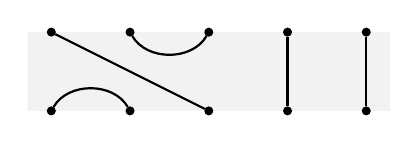
\begin{tikzpicture}
\tikzstyle{blackdot}=[draw=black,circle,fill=black,inner sep=1pt]
\tikzstyle{arrow}=[thick]
\node [blackdot] at (0,0) (u1) {};
\node [blackdot,right of=u1] (u2) {};
\node [blackdot,right of=u2] (u3) {};
\node [blackdot,right of=u3] (u4) {};
\node [blackdot,right of=u4] (u5) {};
\node [blackdot,below of=u1] (d1) {};
\node [blackdot,below of=u2] (d2) {};
\node [blackdot,below of=u3] (d3) {};
\node [blackdot,below of=u4] (d4) {};
\node [blackdot,below of=u5] (d5) {};

\draw [arrow] (u1) edge (d3);
\draw [arrow,bend right=60] (u2) edge (u3);
\draw [arrow,bend right=60] (d2) edge (d1);
\draw [arrow] (u4) edge (d4);
\draw [arrow] (u5) edge (d5);
\begin{pgfonlayer}{background layer}
\fill  [grey] plot (-.3,0) rectangle (4.3,-1);
\end{pgfonlayer}
\end{tikzpicture}

\end{center}
corresponds to (()(()))()
\gap

Applications in Physics: statistical mechanics, percolation problem.

\begin{center}
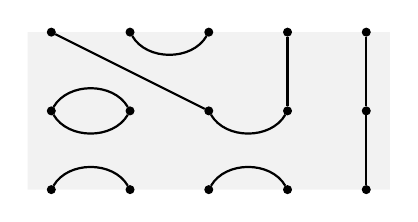
\begin{tikzpicture}
\tikzstyle{blackdot}=[draw=black,circle,fill=black,inner sep=1pt]
\tikzstyle{arrow}=[thick]
\node [blackdot] at (0,0) (u1) {};
\node [blackdot,right of=u1] (u2) {};
\node [blackdot,right of=u2] (u3) {};
\node [blackdot,right of=u3] (u4) {};
\node [blackdot,right of=u4] (u5) {};
\node [blackdot,below of=u1] (d1) {};
\node [blackdot,below of=u2] (d2) {};
\node [blackdot,below of=u3] (d3) {};
\node [blackdot,below of=u4] (d4) {};
\node [blackdot,below of=u5] (d5) {};
\node [blackdot,below of=d1] (x1) {};
\node [blackdot,below of=d2] (x2) {};
\node [blackdot,below of=d3] (x3) {};
\node [blackdot,below of=d4] (x4) {};
\node [blackdot,below of=d5] (x5) {};

\draw [arrow] (u1) edge (d3);
\draw [arrow,bend right=60] (u2) edge (u3);
\draw [arrow,bend right=60] (d2) edge (d1);
\draw [arrow] (u4) edge (d4);
\draw [arrow] (u5) edge (d5);
\draw [arrow,bend right=60] (d1) edge (d2);
\draw [arrow,bend right=60] (d3) edge (d4);
\draw [arrow] (d5) edge (x5);
\draw [arrow,bend left=60] (x1) edge (x2);
\draw [arrow,bend left=60] (x3) edge (x4);
\begin{pgfonlayer}{background layer}
\fill  [grey] plot (-.3,0) rectangle (4.3,-2);
\end{pgfonlayer}
\end{tikzpicture}
=
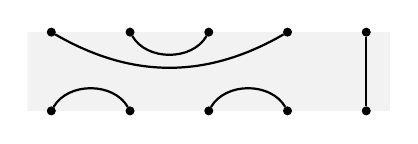
\begin{tikzpicture}
\tikzstyle{blackdot}=[draw=black,circle,fill=black,inner sep=1pt]
\tikzstyle{arrow}=[thick]
\node [blackdot] at (0,0) (u1) {};
\node [blackdot,right of=u1] (u2) {};
\node [blackdot,right of=u2] (u3) {};
\node [blackdot,right of=u3] (u4) {};
\node [blackdot,right of=u4] (u5) {};
\node [blackdot,below of=u1] (d1) {};
\node [blackdot,below of=u2] (d2) {};
\node [blackdot,below of=u3] (d3) {};
\node [blackdot,below of=u4] (d4) {};
\node [blackdot,below of=u5] (d5) {};

\draw [arrow,bend right=30] (u1) edge (u4);
\draw [arrow,bend right=60] (u2) edge (u3);
\draw [arrow,bend right=60] (d2) edge (d1);
\draw [arrow,bend left=60] (d3) edge (d4);

\draw [arrow] (u5) edge (d5);
\begin{pgfonlayer}{background layer}
\fill  [grey] plot (-.3,0) rectangle (4.3,-1);
\end{pgfonlayer}
\end{tikzpicture}
\end{center}
\end{frame}



\begin{frame}
\begin{center}\Huge Thank You!\end{center}
\end{frame}


\end{document}

%%% Local Variables:
%%% mode: latex
%%% TeX-master: t
%%% End:
